% !Mode:: "TeX:UTF-8"
%%%%%%%%%%%%%%%%%%%%%%%%%%%%%%%%%%%%%%%%%%%%%%%%%%%%%%%%%%%%%%%%%%%%%%%%%%%%%%%%
%          ,
%      /\^/`\
%     | \/   |                CONGRATULATIONS!
%     | |    |             SPRING IS IN THE AIR!
%     \ \    /                                                _ _
%      '\\//'                                               _{ ' }_
%        ||                     hithesis v3                { `.!.` }
%        ||                                                ',_/Y\_,'
%        ||  ,                   dustincys                   {_,_}
%    |\  ||  |\          Email: yanshuoc@gmail.com             |
%    | | ||  | |            https://yanshuo.name             (\|  /)
%    | | || / /                                               \| //
%    \ \||/ /       https://github.com/dustincys/hithesis      |//
%      `\\//`   \\   \./    \\ /     //    \\./   \\   //   \\ |/ /
%     ^^^^^^^^^^^^^^^^^^^^^^^^^^^^^^^^^^^^^^^^^^^^^^^^^^^^^^^^^^^^^^
%%%%%%%%%%%%%%%%%%%%%%%%%%%%%%%%%%%%%%%%%%%%%%%%%%%%%%%%%%%%%%%%%%%%%%%%%%%%%%%%
\documentclass[fontset=fandol,type=master,campus=harbin]{hithesisbook}
% 此处选项中不要有空格
%%%%%%%%%%%%%%%%%%%%%%%%%%%%%%%%%%%%%%%%%%%%%%%%%%%%%%%%%%%%%%%%%%%%%%%%%%%%%%%%
% 必填选项
% type=doctor|master|bachelor|postdoc
%%%%%%%%%%%%%%%%%%%%%%%%%%%%%%%%%%%%%%%%%%%%%%%%%%%%%%%%%%%%%%%%%%%%%%%%%%%%%%%%
% 选填选项(选填选项的缺省值已经尽可能满足了大多数需求,除非明确知道自己有什么
% 需求)
% campus=shenzhen|weihai|harbin
%   含义:校区选项,默认harbin
% glue=true|false
%   含义:由于我工规范中要求字体行距在一个闭区间内,这个选项为true表示tex自
%   动选择,为false表示区间内一个最接近版心要求行数的要求的默认值,缺省值为
%   false。
% tocfour=true|false
%   含义:是否添加第四级目录,只对本科文科个别要求四级目录有效,缺省值为
%   false
% fontset=windows|mac|ubuntu|fandol|adobe
%   含义:设置字体,默认情况会自动识别系统,然后设置字体。后两个是开源字体,自行
%   下载安装后设置使用。windows是中易字库,窝工默认常用字体,绝对没毛病。mac和
%   ubuntu 默认分别是华文和思源字库,理论上用什么字库都行。后两种开源字库的安装
%   方法到谷歌上百度一下什么都有了。Linux非ubuntu发行版、非x86架构机器等如何运行
%   可到github issue上讨论。
% tocblank=true|false
%   含义:目录中第一章之前,是否加一行空白。缺省值为true。
% chapterhang=true|false
%   含义:目录的章标题是否悬挂居中,规范中要求章标题少于15字,所以这个选项
%   有无没什么用,除了特殊需求。缺省值为true。
% fulltime=true|false
%   含义:是否全日制,缺省值为true。非全日制如同等学力等,要在cover中设置类
%   型,封面中不同格式
% subtitle=true|false
%   含义:论文题目是否含有副标题,缺省值为false,如果有要在cover中设置副标
%   题内容,封面中显示。
% newgeometry=one|two|no
%   含义:规范中的自相矛盾之处,版芯是否包含页眉页脚,旧方法是按照包含页眉
%   页脚来设置。该选项是多选选项,如果设置为no,则版新为旧模板的版芯设置方法,
%   如果设置该选项one或two,分别对应两种页眉页码对应版芯线的相对位置。第一种
%   是严格按照规范要求,难看。第二种微调了页眉页码位置,好一点。默认two。
% debug=true|false
%   含义:是否显示版芯框和行号,用来调试。默认否。
% openright=true|false
%   含义:博士论文是否要求章节首页必须在奇数页,此选项不在规范要求中,按个
%   人喜好自行决定。 默认否。注意,窝工的默认情况是打印版博士论文要求右翻页
%   ,电子版要求非右翻页且无空白页。如果想DIY(或身不由己DIY)在什么地方右
%   翻页,将这个选项设置为false,然后在目标位置添加`\cleardoublepage`命令即
%   可。
% library=true|false
%   含义:是否为提交到图书馆的电子版。默认否。注意:如果设置成true,那么
%   openright选项将被强制转换为false。
% capcenterlast=true|false
%   含义:图题、表题最后一行是否居中对齐(我工规范要求居中,但不要求居中对
%   齐),此选项不在规范要求中,按个人喜好自行决定。默认否。
% subcapcenterlast=true|false
%   含义:子图图题最后一行是否居中对齐(我工规范要求居中,但不要求居中对齐
%   ),此选项不在规范要求中,按个人喜好自行决定。默认否。
% absupper=true|false
%   含义:中文目录中的英文摘要在中文目录中的大小写样式歧义,在规范中要求首
%   字母大写,在work样例中是全大写。该选项控制是否全大写。默认否。
% bsmainpagenumberline=true|false
%   含义:由于本科生论文官方模板的页码和页眉格式混乱,提供这个选项自定义设
%   置是否在正文中显示页码横线,默认否。
% bsfrontpagenumberline=true|false
%   含义:由于本科生论文官方模板的页码和页眉格式混乱,提供这个选项自定义设
%   置是否在前文中显示页码横线,默认否。
% bsheadrule=true|false
%   含义:由于本科生论文官方模板的页码和页眉格式混乱,提供这个选项自定义设
%   置是否显示页眉横线,默认显示。
% splitbibitem=true|false
%   含义:参考文献每一个条目内能不能断页,应广大刀客要求添加。默认否。
% newtxmath=true|false
%   含义:数学字体是否使用新罗马。默认是。
% chapterbold=true|false
%   含义:本科生章标题在目录和正文中是否加粗
% engtoc=true|false
%   含义:非博士生需要添加英文目录的,手动添加,如果是博士,此开关无效
% zijv=word|regu
%   含义:字距设置为规范规定33个字还是word中34个字。默认regu。
%%%%%%%%%%%%%%%%%%%%%%%%%%%%%%%%%%%%%%%%%%%%%%%%%%%%%%%%%%%%%%%%%%%%%%%%%%%%%%%%
\usepackage{hithesis}

\graphicspath{{figures/}}

\begin{document}
\frontmatter
% !Mode:: "TeX:UTF-8"

\hitsetup{
  %******************************
  % 注意:
  %   1. 配置里面不要出现空行
  %   2. 不需要的配置信息可以删除
  %******************************
  %
  %=====
  % 秘级
  %=====
  statesecrets={公开},
  natclassifiedindex={TM301.2},
  intclassifiedindex={62-5},
  %
  %=========
  % 中文信息
  %=========
  ctitlecover={基于虚拟物理仿真思考的开放任务求解},%放在封面中使用,自由断行
  ctitle={基于虚拟物理仿真思考的开放任务求解},%放在原创性声明中使用
  cxueke={工程},
  csubject={软件工程},
  caffil={计算学部},
  cauthor={柴士童},
  csupervisor={范晓鹏},
  % 日期自动使用当前时间,若需指定按如下方式修改:
  cdate={2020年12月},
  cstudentid={18S103239},
  cstudenttype={全日制工程硕士}, %非全日制教育申请学位者
  %cnumber={no9527}, %编号
  %cpositionname={哈铁西站}, %博士后站名称
  %cfinishdate={20XX年X月---20XX年X月}, %到站日期
  %csubmitdate={20XX年X月}, %出站日期
  %cstartdate={3050年9月10日}, %到站日期
  %cenddate={3090年10月10日}, %出站日期
  %(同等学力人员)、(工程硕士)、(工商管理硕士)、
  %(高级管理人员工商管理硕士)、(公共管理硕士)、(中职教师)、(高校教师)等
  %
  %
  %=========
  % 英文信息
  %=========
  etitle={Physical Simulation and Reasoning based Task-Agnostic learning},
  exueke={Technology},
  esubject={Software Engineering},
  eaffil={\emultiline[t]{Faculty of Computing}},
  eauthor={CHAI Shitong},
  esupervisor={Professor FAN Xiaopeng},
  %eassosupervisor={XXX},
  % 日期自动生成,若需指定按如下方式修改:
  edate={December, 2020},
  estudenttype={Master of Engineering},
  %
  % 关键词用“英文逗号”分割
  ckeywords={元学习, 强化学习, 机器人学, 物理仿真, 深度学习},
  ekeywords={Meta Learning, Reinforcement Learning, Robotics, Physics Simulation, Deep Learning},
}

\begin{cabstract}
本文在Pyrobolearn机器人仿真环境中设计了一个要求机械臂的末端执行器到达指定物体附近的开放任务,并设计了新的强化学习算法用于训练智能体在未获得任务相关的奖励之前在未知环境中学习到可泛化到该开放任务的策略。

在TD3算法和HER算法的基础上,本文引入了基于局部敏感哈希的基于计数的奖励和基于正向动力学预测的奖励用于鼓励智能体探索未知环境。并提出了高斯混合噪声层、和基于物理仿真引擎的奖励。


本文提出的斯混合噪声层被用于提供自适应的策略噪声。本文提出的基于物理仿真引擎仿真时间的奖励被用于在未知任务的环境中鼓励智能体学习有效可泛化的策略,并在获得稀疏奖励的开放任务后快速适应到新的策略。

\end{cabstract}

\begin{eabstract}
A task which requires the end effector of a manipulator to reach a specific body is designed with the help of the robot learning framework Pyrobolearn. New reinforcement learning algorithms are proposed to train an agent to learn in a task-agnostic environment without reward related to the task, where the learnt policy of the agent should be generalizable to the proposed task.

Based on TD3 and HER algorithms, a locality sensitive hashing based reward and a forward dynamics prediction model based reward are introduced to encourage the agent to explore in the unknown environment. A mixed gaussian noise layer is proposed to provide a adaptive policy noise. A reward based on physics simulation time is proposed to encourage the agent to learn a generalizable policy in a task agnostic environment, and adapt to a new policy after given a task setting with sparse reward.
\end{eabstract}
 % 封面
\makecover
\tableofcontents %目录
\mainmatter
\chapter{绪论}

    \section{选题背景及研究意义}
    
        \subsection{选题背景}
        一直以来,强化学习和机器人学都是人工智能研究中的热门领域。在2008年,Deepmind团队基于深度强化学习研发的围棋人工智能系统AlphaGo Zero在零知识自我对弈的情况下在几天之内超越了旧的系统AlphaGo,而AlphaGo曾击败了围棋领域中世界公认的专家柯洁等人\cite{silver2018general}。这项研究使越来越多的人们开始关注人工智能领域,并使得强化学习成为研究热点。事实上,强化学习已经成为最热门的研究领域之一,并在自动控制、运筹学、机器人学、游戏智能体和无人驾驶等领域中获得了广泛的应用\cite{dosovitskiy2017carla}。在这些领域中,机器人学是和前沿强化学习算法关系最密切的领域之一。传统的机器人如机械臂、四足机器人等,可以用强化学习训练得到的智能体进行控制,并在与环境交互过程中根据环境反馈使策略得到进一步的优化。

        然而,由于机器人设计和制造的成本较高,通用的多关节机器人通常非常昂贵。而且机器人通常容易在强化学习中的各种随机探索中受到损坏,并导致控制系统和智能体策略在训练过程中出现错误。因此在实际的机器人上进行所有强化学习训练是不现实的\cite{toussaint2018differentiable, todorov2012mujoco}。为了避免这个问题,可以使用物理仿真引擎对机器人和环境进行建模,并在实际测试智能体之前先在仿真环境中对智能体进行训练。幸运的是,随着强化学习仿真需求的增加,越来越多的针对机器人的仿真环境开始出现,在这些仿真环境中,可以像在真实环境中一样控制机器人的关节、调节各种参数,或获得传感器数据等等,并可以做到在真实环境中难以做到的设定复杂的稀疏奖励、获取碰撞次数、和改变环境的物理参数等操作\cite{savva2019habitat}。

        虽然已经有大量的软件系统可以用于在一个环境建模完全精确的情形下解决一个良定义的任务\cite{toussaint2018differentiable},如何让智能体在面对未知的新环境和未知的新任务后能够有效泛化之前学习到的策略仍然是一个未完全解决的问题。人类可以在陌生的环境中用很少次数的探索自然地掌握大量有效信息,还可以利用已有经验对大量物体进行分类、提高对物理实体运动的预测能力,或创新性地设计工具解决问题。由于人们对大脑的工作原理仍然知之甚少,这个过程通常很难被数值化为一个单一的奖励函数或强化学习算法。

        本课题致力于解决上述问题,即设计算法从而可以训练出能在任务奖励未知的环境中进行探索,获取环境信息,学习基本策略,并在任务确定后快速调节旧策略以适应新任务的智能体。为了实现这个目标,需要利用现有的开源物理仿真引擎、前沿的强化学习算法和具有强大函数拟合能力的深度神经网络来设计新算法。
        
        \subsection{研究意义}

        机器人控制对于工业制造有着重要的意义,在工厂流水线上,机械臂常常被设计为只能完成单个简单任务,或需要工人远程控制。虽然它们已经极大地提高了生产效率,减少了对工人们生命财产安全的威胁,但是机械臂由于价格昂贵,仅仅用于单一任务会造成极大的资源浪费。

        本课题提出的算法有希望训练出可以在对未知任务奖励的环境进行充分探索之后,快速适应多种不同任务的机器人智能体,从而扩大现有强化学习算法的适用范围,解决更复杂的控制任务,增强机器人智能体泛化策略的能力。

        此外,本课题还可以加深对现有强化学习算法在机器人控制中应用价值的理解,可以通过机器人仿真和控制帮助提前发现在应用算法到实际机器人控制时可能出现的问题,可以通过设计和调整深度神经网络进一步了解不同结构的神经网络对智能体性能的影响。
    
    \section{国内外研究进展}

    国内外已经有了很多关于让机器人智能体使用工具和泛化已学习的策略到新任务的研究。其中关注工具使用、无监督兴趣导向的探索、模仿学习和自驱动的主动学习与本课题有关。
        \subsection{基于引导视觉预见的工具使用}
        引导视觉预见\cite{xie2019improvisation}可以使机械臂智能体从人类演示中学习并泛化学习到的能力以在不同的环境中使用工具。这种方法包含动作提案模型和预测模型。其中动作提案模型使用演示动作数据来训练一个自回归的长短时记忆网络模型来根据图像传感器拍摄到的图像数据生成动作。预测模型是基于卷积长短时记忆网络的\cite{shi2015convolutional}。预测模型被用于对物理实体的运动进行物理预测,并可以被用于筛选不能完成指定目标的动作序列。训练过程分为基于演示的模仿学习和利用握爪反射的随机自动训练。在测试过程中,指定的目标被定义为像素移动,预测模型输出的像素位置和真实像素位置的距离被用于评估动作好坏。在指定任务后,动作序列从动作提案模型中采样,并使用交叉熵方法结合预测模型进行优化。实验表明,此种方法可以比单纯模仿学习在新环境中获得更好的泛化性能。

        \subsection{无监督兴趣导向探索}
        引导视觉预见需要有人类使用工具的演示数据才能正常工作,而对于更一般的环境,人类的演示数据可能是无法获得的,此时智能体应当可以在没有指定任务的情况下在环境中探索。为了解决这个问题,一个兴趣导向的探索方法被提出了\cite{laversanne-finot2018curiosity}。这个方法结合了解纠缠目标空间的变分自编码机(VAE)和兴趣导向的IMGEP(Intrinsically Motivated Goal Exploration Process)方法\cite{DBLP:journals/corr/abs-1708-02190}。在目标空间被给定后,IMGEP框架下的智能体会倾向于选择更有可能增加竞争力的目标。因为不像通常的强化学习算法一样在给定单一目标后做训练,而是无监督地选择目标进行训练,因此这是一个元策略算法。在探索过程中,智能体会学习到被$\beta$-VAE解纠缠后的观测,因此智能体可以分离地探索不同的物体。在实验中,此种方法获得了比单纯IMGEP方法更大的探索率。

        \subsection{模仿学习}
        在需要使用工具求解的开放任务中,往往有着稀疏奖励,随机探索很难刚好完成一个完整的动作序列,最终成功地使用工具完成任务,并获得奖励。
        模仿学习通过人类的专家策略,可以极大地加速这种随机探索过程。通过人类提供的演示数据,智能体应当能够学习到更好的探索策略,增大获得奖励的概率。
        相关研究表明,使用常规的强化学习算法和运动剪辑数据集,智能体可以学会组合学到的不同的技能,并用于求解多种任务\cite{peng2018deepmimic}。不仅如此,智能体也可以从视频中学习到一些技能\cite{peng2019sfv}。这意味着现有模仿学习方法可以利用网络中大量的视频数据进行学习。

        \subsection{自驱动的主动学习}
        在开放任务求解中,主动学习技术也可以被使用。为了主动学习预测物理环境的能力,可以使用带策略的循环Q网络来减少未知物理性质的熵\cite{li2019active}。
        在机器人学中,逆动力学模型对于稳健控制非常重要。一种主动学习方法使用竞争力来选择目标并在高维连续空间中学习各种技能,并用于机器人控制\cite{baranes2013active}。仿真结果表明这种方法能够帮助机器人智能体探索到随机策略难以探索到的区域。

    \section{研究内容和方法}

        \subsection{研究内容}

        \subsection{研究方法}


% !Mode:: "TeX:UTF-8"

\chapter{实验环境}

\section{Gym和Pyrobolearn}\label{introenv}
Gym\cite{brockman2016openai}是一个由OpenAI团队开源的强化学习仿真环境,它已经成为了评价最先进的基线强化学习算法或机器人控制算法的标准环境。
Mujoco\cite{todorov2012mujoco}是一个著名的商业物理仿真引擎,它在强化学习和机器人学中得到广泛应用,并成为Gym中机器人相关的环境的默认仿真引擎。
在接下来的几章中,Gym将被用来验证算法正确性,或被用于更方便地与其他现有算法进行对比。

Gym提供一个Python语言的接口并且已经被包含在了Python包检索中。
Gym需要使用OpenGL的开源库GLFW来进行渲染。
它可以直接使用Python包管理器\emph{pip}进行安装。
在Gym中,有很多内置的环境,包含大量著名的和强化学习有关基本任务可用于验证强化学习算法,并提供了统一的接口。
例如,它包含一个经典的名为“推车杆”的控制任务,这个任务要求智能体通过水平地移动推车来平衡一个底部用自由活动的关节连接到推车上的杆。
一个正常的强化学习算法应当可以在较长时间内避免杆失去平衡并倒下。

Mujoco(Multi-Joint dynamics with Cotact)是一个致力于仿真复杂关节运动、碰撞和多物体接触的物理引擎。
它集成了粒子系统仿真、约束求解器、有限元积分器和凸优化器等等工具。
它使用ANSI C编写并有一个Python的API封装。
在Gym中,\emph{FetchReach-v1}环境需要使用Mujoco作为仿真器,因此在实验中Mujoco、OpenGL和Gym等工具都被安装在Ubuntu 20.04系统中,并设置了环境变量以保证正确的动态链接库\emph{libGL.so}和Mujoco的二进制分发被加载。

一个\emph{FetchReach-v1}环境的截图展示在图\ref{fetchreach-v1}中。
    \begin{figure}
        \centering
        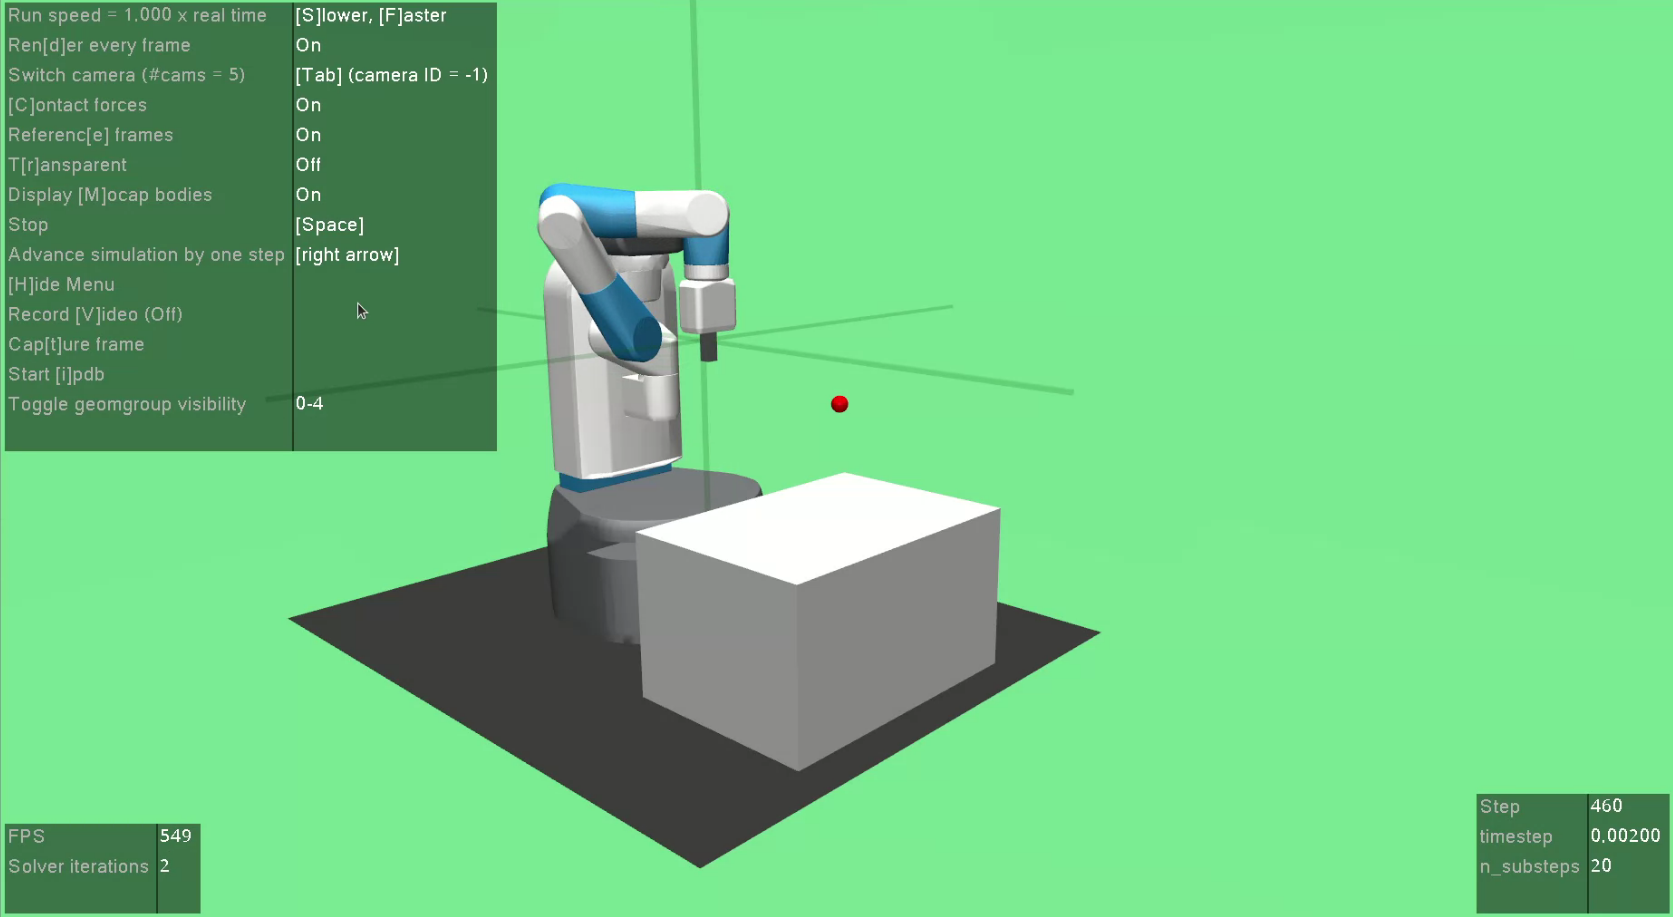
\includegraphics[width=0.5\textwidth]{fetchreach-v1.png}
        \caption{FetchReach-v1环境的截图}
        \label{fetchreach-v1}
    \end{figure}
其中有一个机械臂被放在一张桌子前。
在每个片段刚开始时,这个机械臂的状态都会被重置,而一个红点则会随机地出现在桌子上方的某处。
机械臂智能体需要在片段的限制时间内使自己的末端执行器到达这个红点附近来完成任务并获得奖励。
在片段的每一个时间步中,都会有观测值提供给此机械臂智能体。
观测值包括指示关节状态、末端执行器位置坐标信息作为已完成的目标,和红点的位置坐标信息作为期望目标。
指示关节状态的观测值$o\in \mathbb R^{10}$是一个10维的向量,而末端执行器的坐标$g^a \in \mathbb R^3$和红点的位置坐标$g^d\in\mathbb R^3$都是3维的向量。
因此提供给机械臂智能体的状态向量是一个16维的向量$s=(o, g^a, g^d)\in \mathbb R^{16}$。
如果末端执行器和红点之间的距离小于一个阈值,一个值为0.0的奖励会被提供给机械臂智能体,否则一个值为-1.0的奖励会被提供给它。
机械臂可以采取的动作是一个4维的取值在-1到1之间的向量,即$a\in[-1,1]^4$。

\section{Pyrobolearn和Pybullet}
虽然使用Gym和Mujoco的功能已经可以覆盖本课题的大部分实验,但是由于Mujoco是商业仿真软件,且可定制性不强,因此有必要使用开源的替代品,即Pyrobolearn和Pybullet,来设计本课题中的主体实验。

Pyrobolearn是一个专门设计来训练智能机器人的框架\cite{delhaisse2019pyrobolearn}。
它目前仍然在开发中,但是大部分实验中用到的功能已经足够稳定。
一些尚未在其中实现的功能也可以通过继承现有类来进行自定义。
与Gym相似,Pyrobolearn也有一个默认的物理引擎。
这个物理引擎叫做Pybullet\cite{coumans2016pybullet}。
它是一个C++编写的开源的物理引擎Bullet3在Python接口的封装,并可以提供本文中需要的所有仿真功能。它可以实时地检测碰撞,并可以精确地仿真多物理现象,这保证了它可以被用于本文需要的机器人和物体交互仿真的研究需求。
虽然Pyrobolearn也有一个使用Mujoco作为仿真器的接口,但是它对Mujoco的支持尚未稳定,因此本文的实验选择了使用Pybullet作为仿真器。

使用Pybullet作为仿真器,Pyrobolearn可以被用来仿真多种经典的机器人控制和强化学习问题。
实际使用中,一个物理世界对象包含了一些固定的物理量,例如重力方向和摩擦系数,并可以加载物体和机器人。
一个世界对象在构造过程中通常要提供一个仿真器,本文提供了Pybullet作为仿真器。
在世界对象构造完成后一个由仿真器生成的世界相机会被提供给世界对象作为一个属性。

在接下来的使用Pyrobolearn的实验中,全部都使用了\emph{Basic World}类型的世界对象,其中重力加速度向量为笛卡尔坐标系中的(0.0, 0.0, -9.81),横向摩擦系数为1.0,旋转摩擦系数为0.0,滚动摩擦系数为0.0,线性阻尼为0.04,角阻尼为0.04。

渲染后的世界相机下的\emph{Basic World}世界如图\ref{basicworld}所示。
    \begin{figure}
        \centering
        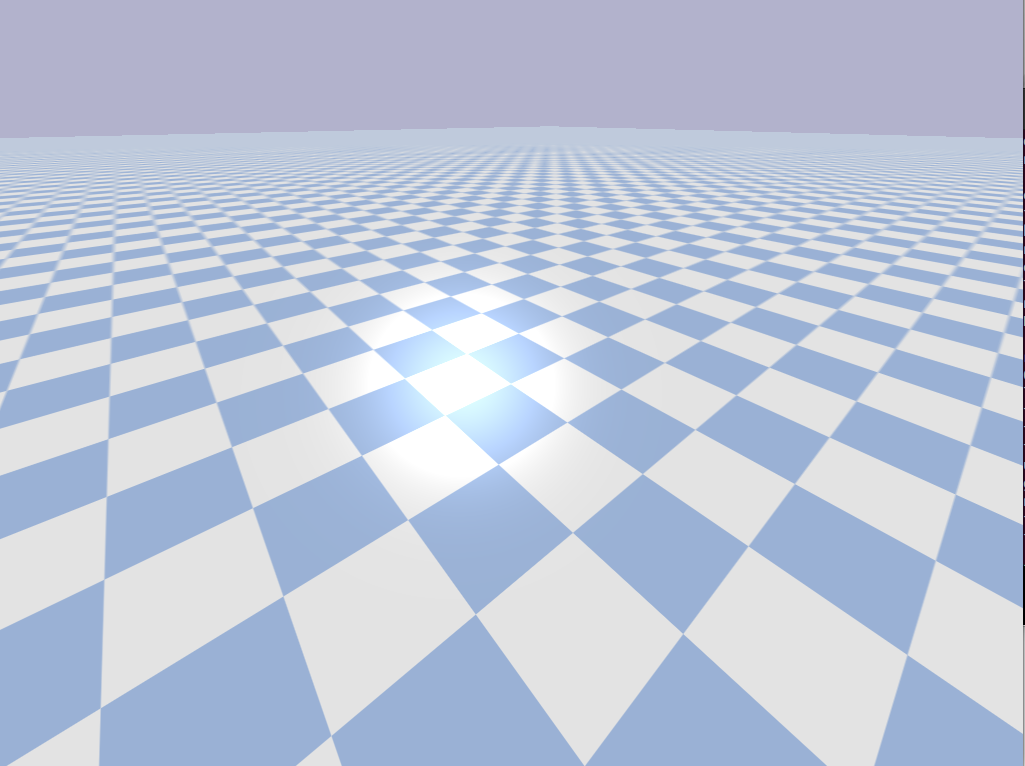
\includegraphics[width=0.3\textwidth]{basicworld.png}
        \caption{空白的\emph{Basic World}世界渲染结果}
        \label{basicworld}
    \end{figure}
默认情况下,没有物体和机器人被加载,只有地面和基本物理量被初始化。

两种不同的机械臂分别在初步实验和主体实验中使用。其中一个来自于Gym环境,另一个来自于Pyrobolearn框架。

在基于Mujoco的几个Gym环境中,一个和Fetch研究平台中的Fetch便携机械臂具有相同参数的机械臂被用作默认的唯一一个与环境交互的机器人\cite{Wise2016FetchF}。
Fetch便携机械臂有7个自由度。
在本文中使用到的\emph{FetchReach-v1}环境中,只有其中的4个被使用。
如第1节所述,\emph{FetchReach-v1}环境中的状态向量由Fetch机械臂的关节的位置信息、末端执行器的笛卡尔坐标和红点的笛卡尔坐标构成。

Pyrobolearn框架中的主体实验使用了一个叫做WAM的机械臂。
WAM机械臂可以配备手指终端执行器,它们一共有15个自由度,这意味着动作空间是非常高维的。
在\emph{Basic World}世界中加载的WAM机器人如图\ref{wam}所示。
    \begin{figure}
        \centering
        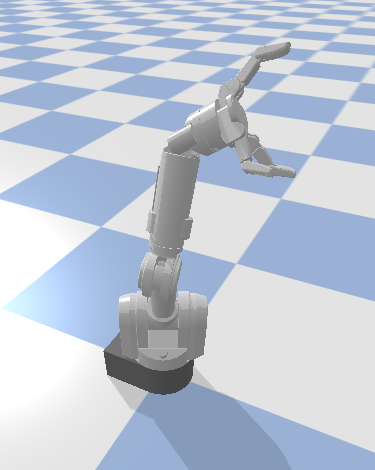
\includegraphics[width=0.3\textwidth]{wam.png}
        \caption{\emph{Basic World}中的WAM机器人渲染结果}
        \label{wam}
    \end{figure}

\section{实验框架}\label{expframe}
本文中所有的实验都有可更改目标的状态,这意味着智能体可以获知当前已完成的目标和期望的目标。
假设期望的目标用一个3维的笛卡尔坐标表示,已完成的目标用机器人的末端执行器的笛卡尔坐标表示。
通常情况下,当这两个坐标间的距离小于一个阈值时,表示任务已经顺利完成。

形式化地,一个状态向量$s\in\mathcal S$是一个由3个向量构成向量,即$s=(o,g^a,g^d)$,其中$o$是观测到的环境中的物理量构成的向量,$g^a$是已完成的目标,$g^d$是期望的目标。
一个环境奖励函数$reward:\mathcal S\to \mathbb R$是由环境反馈决定的智能体在交互中可获得的奖励。

在实验中,因为目标可以方便地修改,所以可以使用事后经验重放算法,这也使得定义具有稀疏奖励的开放任务,并在其中使用多种方法训练高探索效率和泛化能力的智能体成为可能。

智能体与环境的交互在实验中被组织为分离的片段。
每个片段都有相同的最大时间步数$T$。
智能体应当在最大时间步数的限制$t\leq T$下完成一个特定的开放任务并获得较高的奖励。
对于\emph{FetchReach-v1}环境,最大的时间步数为50.
对于在Pyrobolearn框架下的主体实验中自定义的环境中,最大的时间步数为100或200.
智能体可以把在交互中获得的迁移信息$(s_t,a_t,r_t,s_{t+1})$保存在重放缓存中以便之后采样和训练。

对每个片段,最后一个时间步的下一个状态$s_{T+1}$不应被用于训练,因为当环境处理这个状态时这个片段已经结束,因此它不会导致未来的任何奖励。
为了防止在训练过程中使用这个状态,可以引入一个掩膜变量$m$,并与根据$s_{t+1}$计算得出的动作价值函数值相乘。
当$t<T$时,令$m=1$,当达到最后一个时间步,即$t=T$时,令$m=0$,并将$m$和迁移信息一同放入重放缓存中以便训练时与上述动作价值函数相乘。

在每个实验的片段开始时都引入了随机初始化。

对于\emph{FetchReach-v1}环境中的实验,在片段的第一个时间步之前,Fetch便携机械臂的关节位置被初始化为一个固定的起始位置,由红点表示的期望目标则随机地初始化为桌面上的一个位置。

在自定义的Pyrobolearn环境中,在片段开始之前,WAM机械臂上的关节位置被随机初始化,期望的目标也被随机地初始化在1米以内,其中目标的$z$坐标被初始化为0.5,$x,y$则从$[-1,1]$的均匀随机分布中采样。
与\emph{FetchReach-v1}环境中相比,自定义的环境中机械臂的初始状态是随机的,这会给此开放任务带来更多的复杂性。
有时候WAM机械臂的随机初始状态距离目标非常远,这会导致任务理论上不可能完成。

\section{Gym初步实验系统设计}

Gym环境下的实验程序按照类图\ref{gymuml}所示的方式组织。
    \begin{figure}
        \centering
        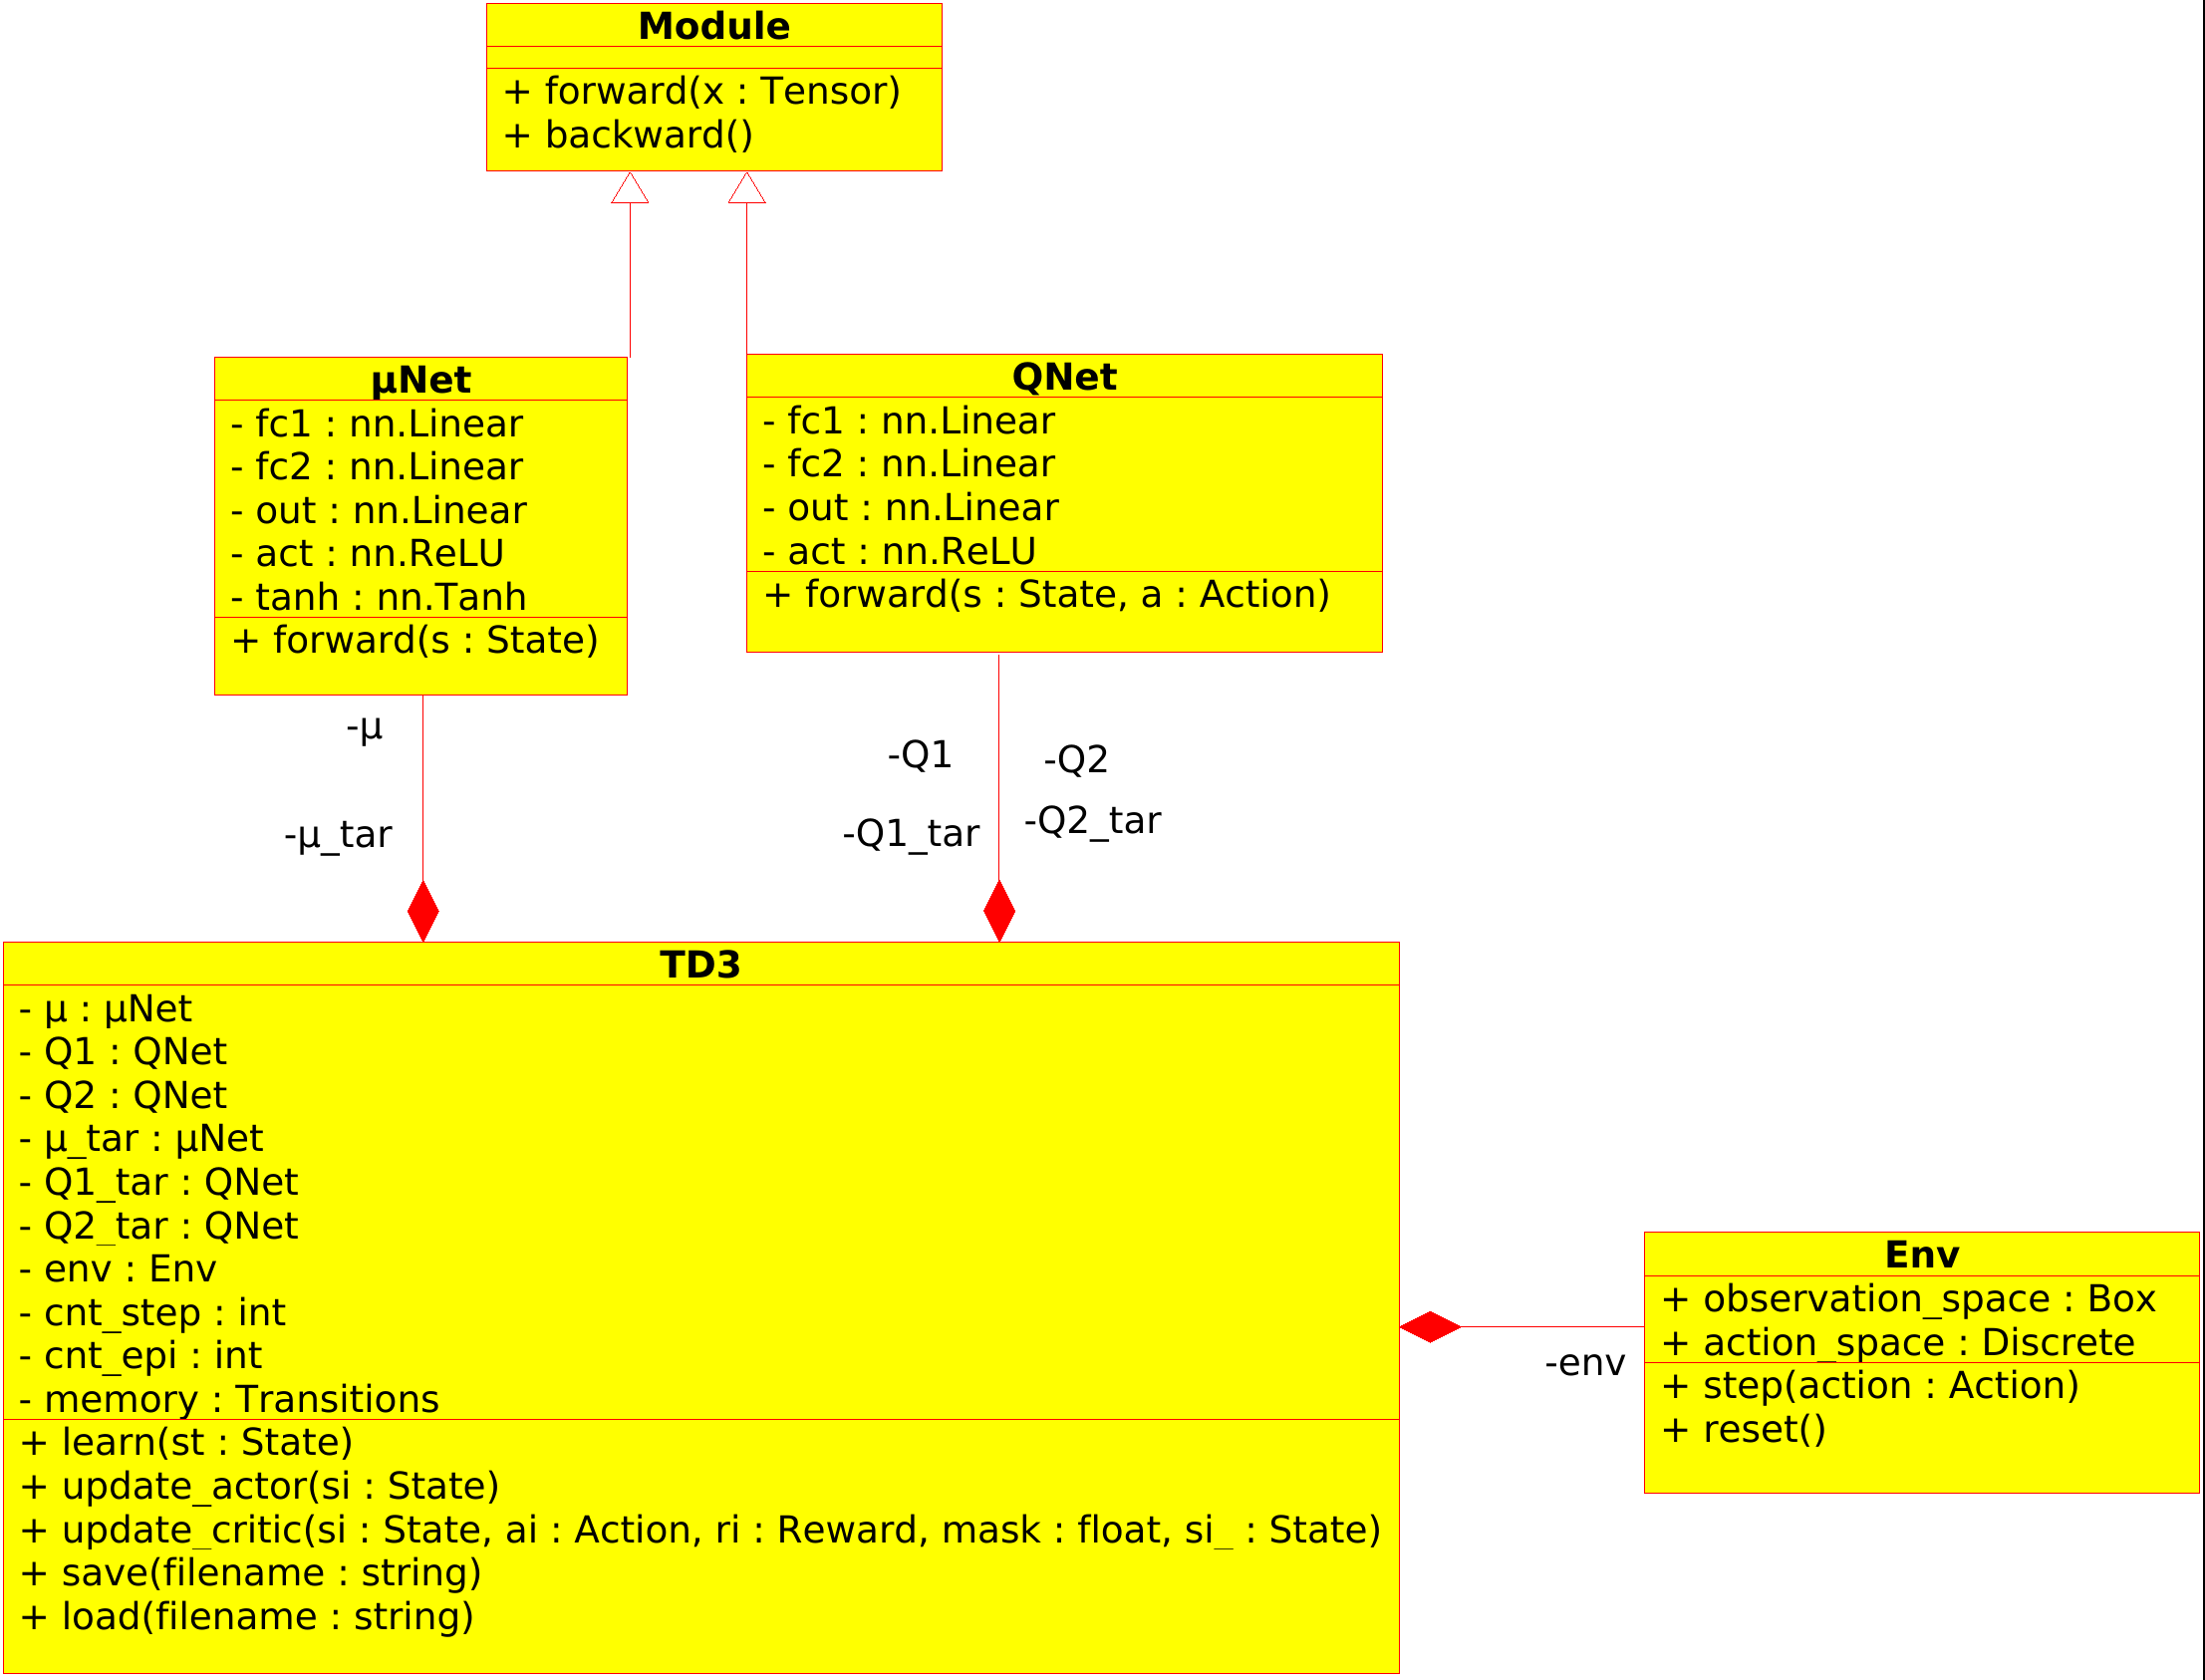
\includegraphics[width=0.6\textwidth]{gymuml.png}
        \caption{Gym初步实验程序类图}
        \label{gymuml}
    \end{figure}
其中Module是Pytorch中的神经网络模块,μNet和QNet通过继承自动获得反向传播的方法backward。
$\mu$,Q1和Q2分别是演员网络,评论家网络1和评论家网络2;$\mu$\_tar,Q1\_tar和Q2\_tar分别是对应的靶网络。
每调用一次TD3对象的learn方法,都会进行一个时间步的仿真,时间步计数器cnt\_step和片断计数器cnt\_epi相当地进行自增运算,并把生成的迁移$(s_t,a_t,r_t,mask_t,s_{t+1})$存入重放缓冲memory中。

上述仿真过程是通过调用环境对象env的step方法来实现的,step方法接收根据演员网络在接收当前状态$s_t$后输出的动作结合相应随机策略生成的动作$a_t$,进行一个时间步的仿真,并输出下一个状态$s_{t+1}$,奖励值$r_t$,此片断是否已经结束$done$和其他信息。
在\ref{expframe}中所述的掩膜$m$可以与折扣系数$\gamma$合并,根据如下公式计算新的掩膜:
\[
m=\begin{cases}
          0, & \text{若} done=True \\
          \gamma, & \text{其他}
\end{cases}
\]

当cnt\_step和cnt\_epi满足一定条件时,update\_actor方法或update\_critic方法会被触发。
在update\_actor和update\_critic方法中,首先对重放缓冲memory进行采样,采样后对采集到的批次迁移数据根据\ref{HERsec}中描述的过程进行事后经验重放。
最后使用如下损失函数计算梯度并用反向传播更新网络权重:
\begin{align}
    & L_\mu = -\sum_i^N\frac{Q_1(s_i, \mu(s_i))}{N} \\
    & L_{Q_1} = \sum_i^N\frac{r_i + m \min\{Q_1'(s_{i+1},\mu(s_{i+1})), Q_2'(s_{i+1},\mu(s_{i+1}))\} - Q_1(s_i,a_i)}{N}\\
    & L_{Q_2} = \sum_i^N\frac{r_i + m \min\{Q_1'(s_{i+1},\mu(s_{i+1})), Q_2'(s_{i+1},\mu(s_{i+1}))\} - Q_2(s_i,a_i)}{N}
\end{align}
其中$\mu, Q_1, Q_2, \mu', Q_1',Q_2'$ 分别对应前述$\mu$,Q1,Q2,$\mu$\_tar,Q1\_tar和Q2\_tar。
为保证实验结果可复现,在经过多次迭代之后要使用save方法保存网络权重,并在测试时使用load方法加载。

上述Q1网络,Q2网络,Q1\_tar网络和Q2\_tar网络都具有相同的网络结构,它们的网络结构如图\ref{gymQnet}所示。

    \begin{figure}
        \centering
        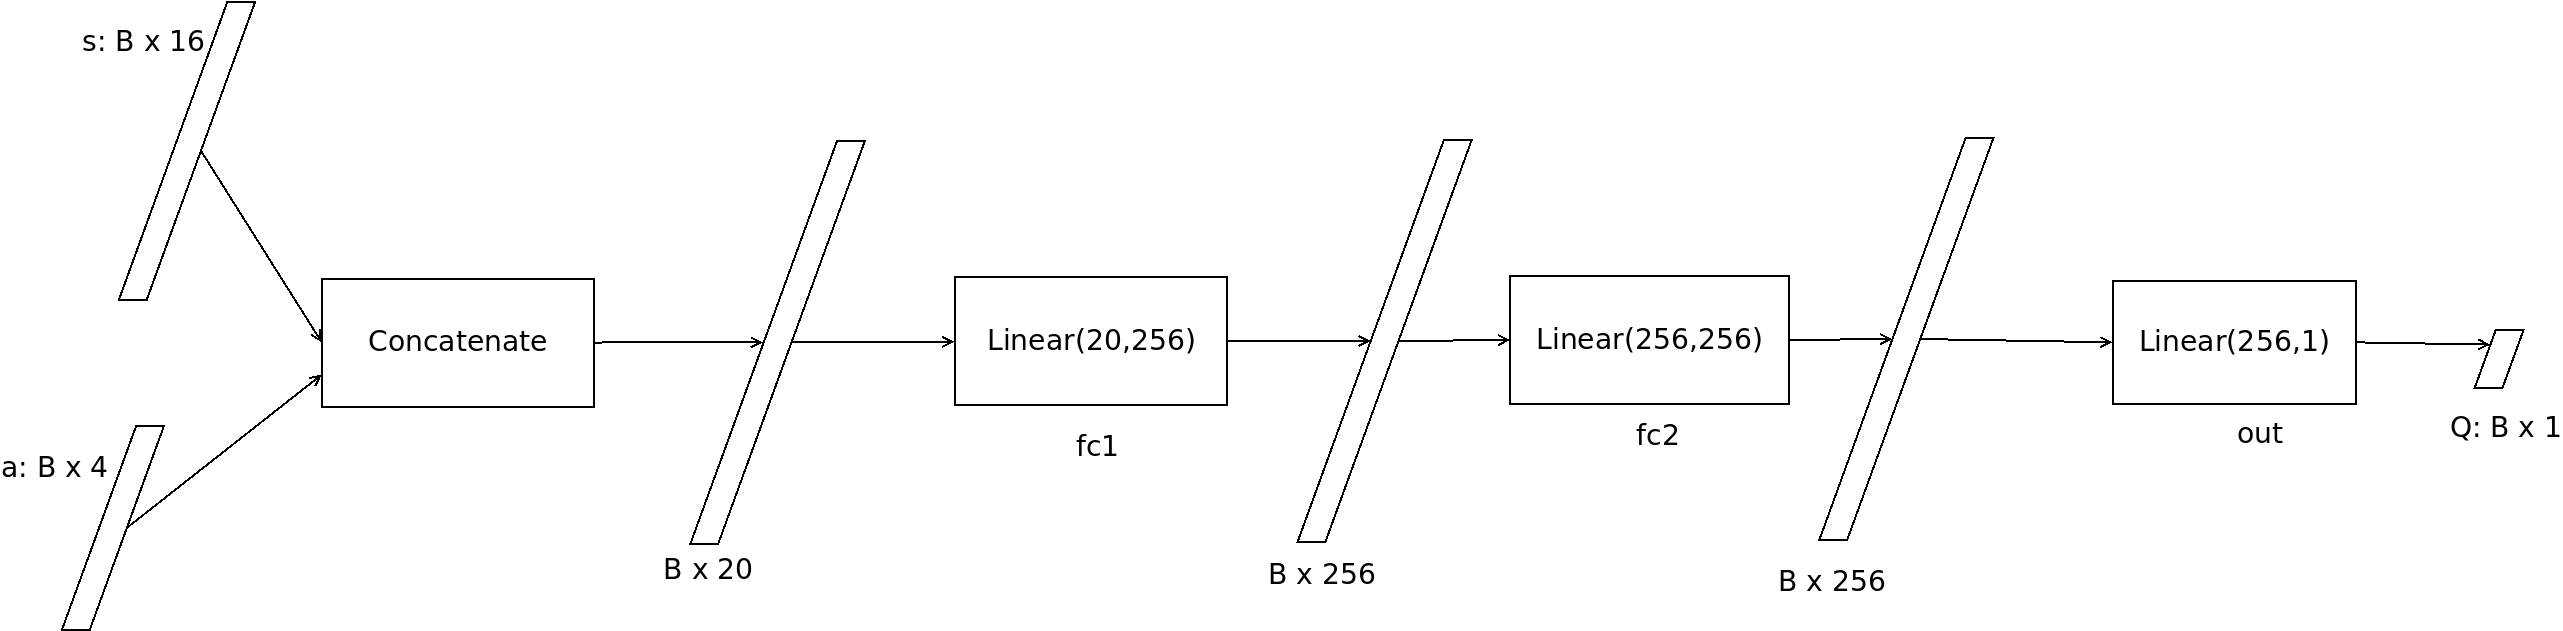
\includegraphics[width=\textwidth]{gymQnet.png}
        \caption{Gym环境下初步实验的评论家网络结构}
        \label{gymQnet}
    \end{figure}

上述$\mu$网络和$\mu$\_tar网络具有相同的网络结构,其网络结构如图\ref{gymMunet}所示。
    \begin{figure}
        \centering
        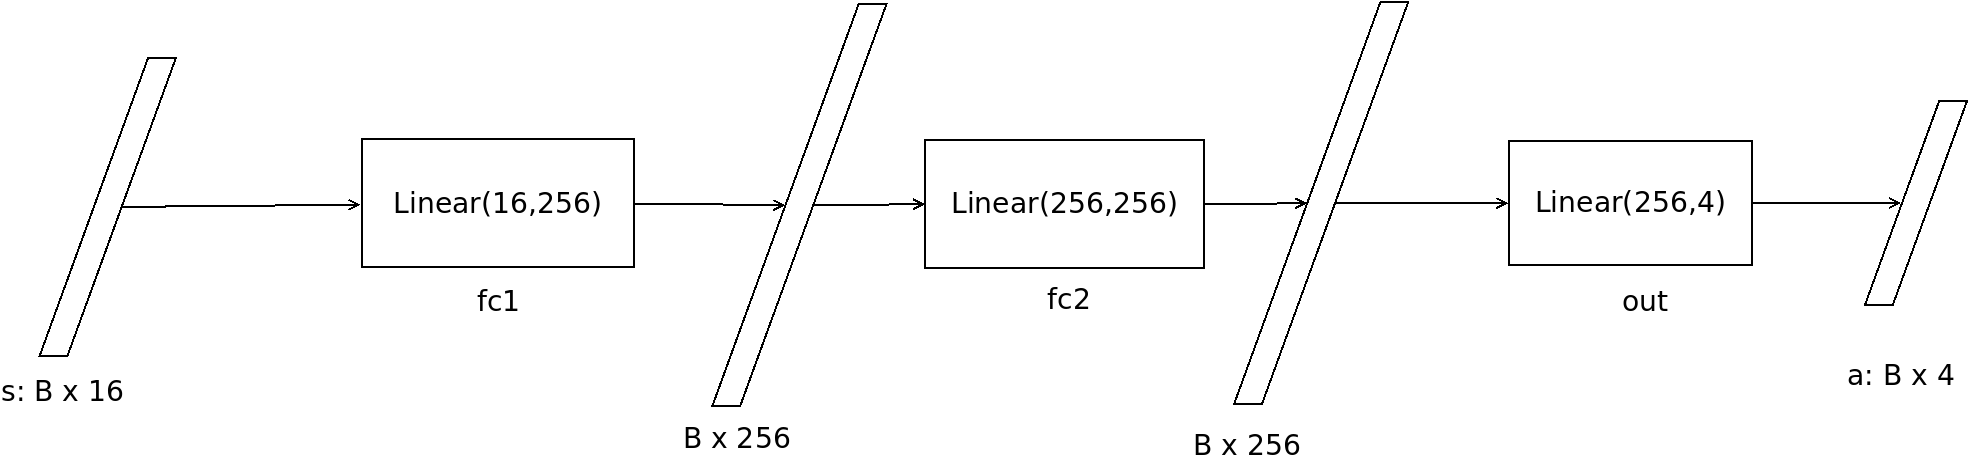
\includegraphics[width=\textwidth]{gymMunet.png}
        \caption{Gym环境下初步实验的演员网络结构}
        \label{gymMunet}
    \end{figure}

\section{Pyrobolearn主体实验系统设计}
在Pyrobolearn框架中自定义的环境中有3种不同类型的状态构成了最终的状态向量:零件(link)世界速度状态、零件世界位置状态和物体位置状态。
在Pyrobolearn中,世界中的对象和机器人都被叫做物体(body)。
每个物体都有一个唯一的物体ID,它可以被世界对象用来找到对应的状态。
而机器人上面互相连接的构件被叫做零件(link)。
每个零件也有一个唯一的零件ID,它可被机器人对象用来找到对应的信息,而不能被世界对象直接访问。
零件的状态必须使用零件的ID来生成,使用物体ID生成零件状态或用零件ID生成物体状态都会导致严重的隐藏错误。

在实验中,WAM机械臂的末端执行器的ID可以使用get\_end\_effector\_ids来得到,而最后一个末端执行器的ID将在实验中用来生成已完成的目标向量$g^a$。
机器人上的一个零件的零件世界位置状态是一个3维的向量,而一个零件的零件世界速度状态是一个6维的向量。
如上所述,在实验中,直接把WAM机械臂的最后一个末端执行器的ID提供给了零件世界位置状态对象的构造方法,此状态对象可以用于监控已完成的目标向量$g^a$的值。
除了上述被选中的最后一个末端执行器,WAM机械臂还有20个其他零件。
每一个零件都有一个3维的世界位置状态和一个6维的世界速度状态。

实验中会有两个物体加载进\emph{Basic World}世界中,一个是上述WAM机械臂,另一个是一个初始位置随机的蓝色方块。
主体实验定义的开放任务为,WAM机械臂的最后一个末端执行器距离蓝色方块的距离应当在片段的最大时间步数限制内缩小到小于一个阈值,在每一个时间步,如果距离大于此阈值,则提供-1.0的奖励,否则提供0.0的奖励。
为了方便使用事后经验重放算法,需要在每个时间步获得蓝色方块的世界位置,用于监控这个期望目标向量$g^d$的状态可以很容易地使用方块的物体ID和物体世界位置构造方法来得到。

上文已经介绍了构成状态向量$s=(o, g^a, g^d)$中的已完成的目标$g^a$和期望目标$g^d$的定义,余下的$o$定义为WAM机械臂上的除了最后一个末端执行器的其他零件的世界位置和世界速度。
最终,这些状态构成了一个192维的状态向量$s\in \mathbb R^{192}$。
主体实验中使用到的这些状态并不是所有的状态。
根据通用机器人描述格式(Universal Robotic Description Format)中描述的模型,还有其他的状态(如图像传感器状态)可以被添加,但是现有的状态信息已经足够多以使得机械臂能够完成此开放任务,因此实验中没有添加更多状态。

在主体实验中,只使用了关节位置变化类型的动作作为机械臂与环境交互的动作。
在机械臂做出一个关节位置变化动作之后,关节的位置与动作值相加即可得到新的关节位置。
关节位置动作是一个15维的向量,这与\emph{FetchReach-v1}环境中的动作维度要高得多,因此在Pyrobolearn中自定义的此开放任务要比前者更难。

所有的实验中用到的动作和状态都是连续的,当考虑到状态空间和动作空间都是连续的这一事实后,可以知道智能体要搜索的空间是非常巨大的,这与上文定义的稀疏奖励结合起来就引出了在此开放任务下探索策略的问题。
在接下来的实验中,多个探索策略被提出以获得更高效率的探索,并更好地解决此问题。

Pyrobolearn下的实验程序的类图如图\ref{myenvuml}所示。
    \begin{figure}
        \centering
        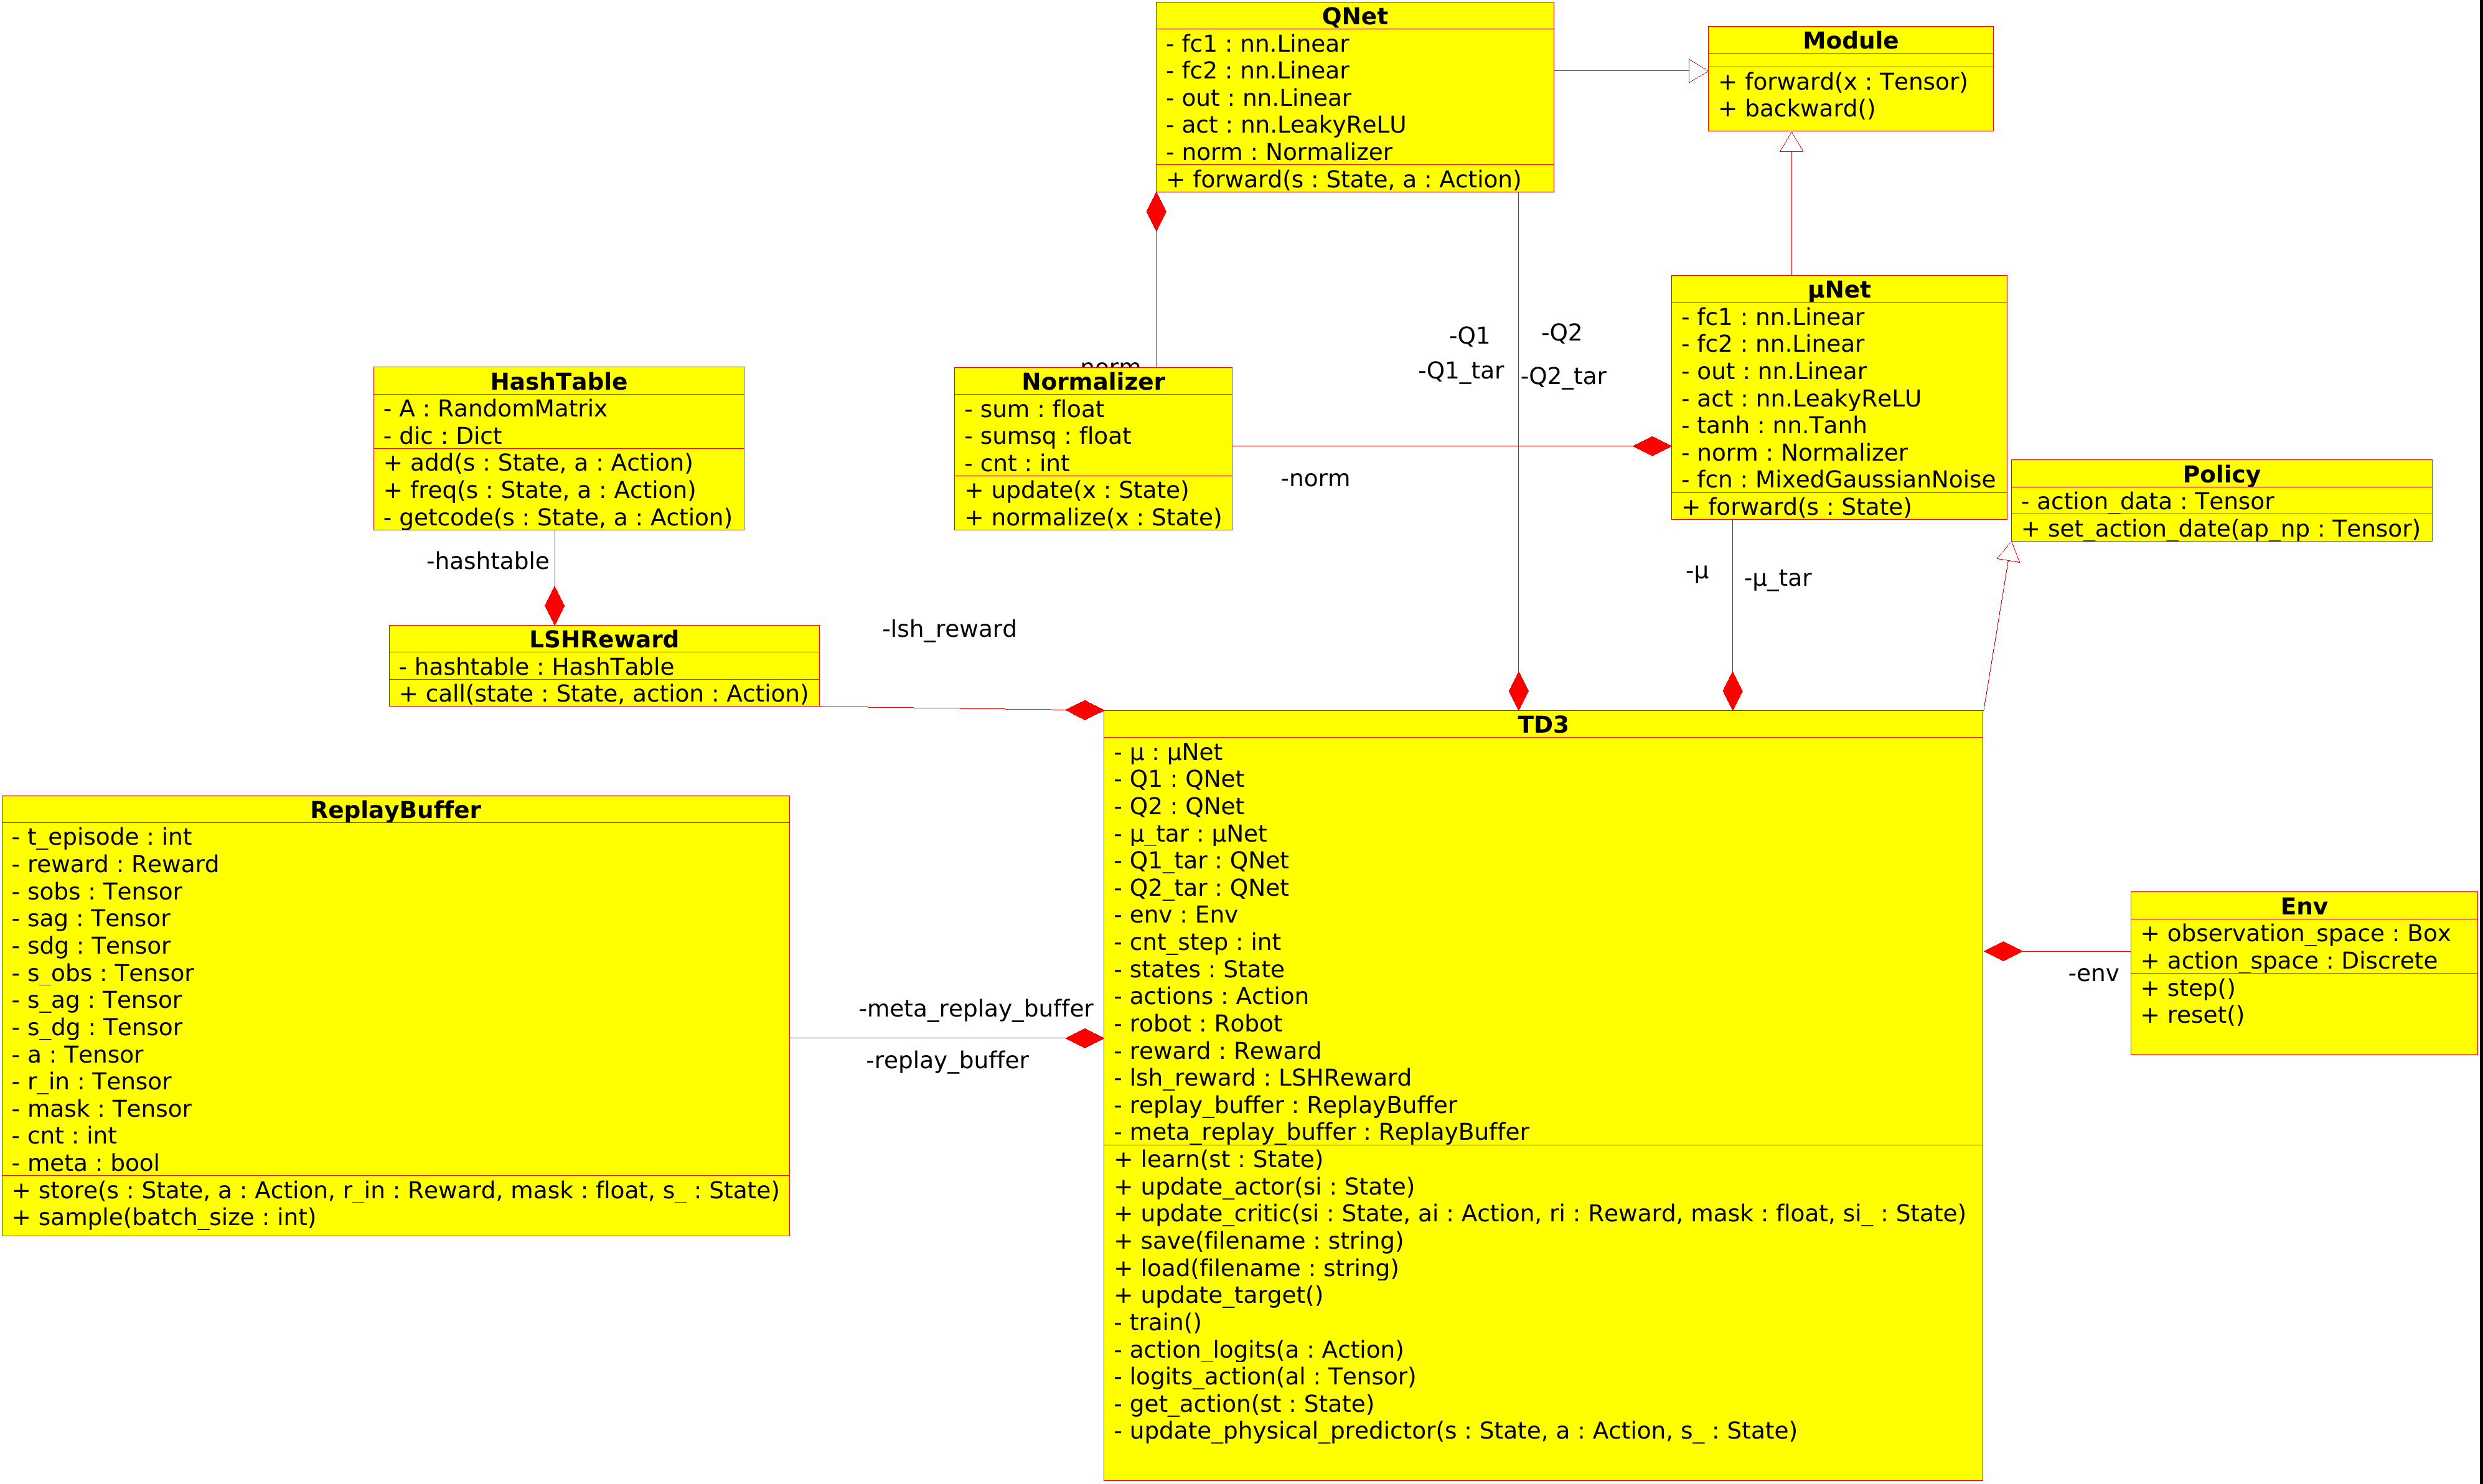
\includegraphics[width=\textwidth]{myenvuml.png}
        \caption{Pyrobolearn主体实验程序类图}
        \label{myenvuml}
    \end{figure}
    其与Gym环境中的初步实验程序的主要区别在于引入了基于局部敏感哈希的内部奖励函数对象LSHReward,正态化器Normalizer,Leaky ReLU激活层,高斯噪声层MixedGaussianNoise和元重放缓冲meta\_replay\_buffer的引入。
    元重放缓冲用于在$t<T_{start}$的时间内,未提供环境奖励时,保存内部奖励对应的迁移。
    另外在其中一个主体实验中还使用了update\_physical\_predictor方法来对正向动力学预测模型进行更新和训练,其中此模型的损失被用于构成内部奖励。
    为了方便演员网络使用Tanh激活层输出,策略TD3中还引入了action\_logits来把动作向量的每个元素的值都缩放到[-1,1],并使用logits\_action来进行反向解码出动作。

    与初步实验中类似,主体实验也使用全连接网络,但在演员网络中最后一层加入了混合高斯噪声层并与原网络输出动作求和,并且对输入层输出层进行了相应调整以适应输入数据。
    由于输入输出主体实验中所有神经网络的动作向量都进行了缩放,演员网络的最后一层不需要再乘以max\_action,只需要直接输出[-1,1]的缩放后的动作值,在策略TD3中调用演员网络的地方会自动进行缩放。

    主体实验中使用的演员网络结构如图\ref{myenvMunet}所示。
    主体实验中使用的评论家网络结构如图\ref{myenvQnet}所示。
    \begin{figure}
        \centering
        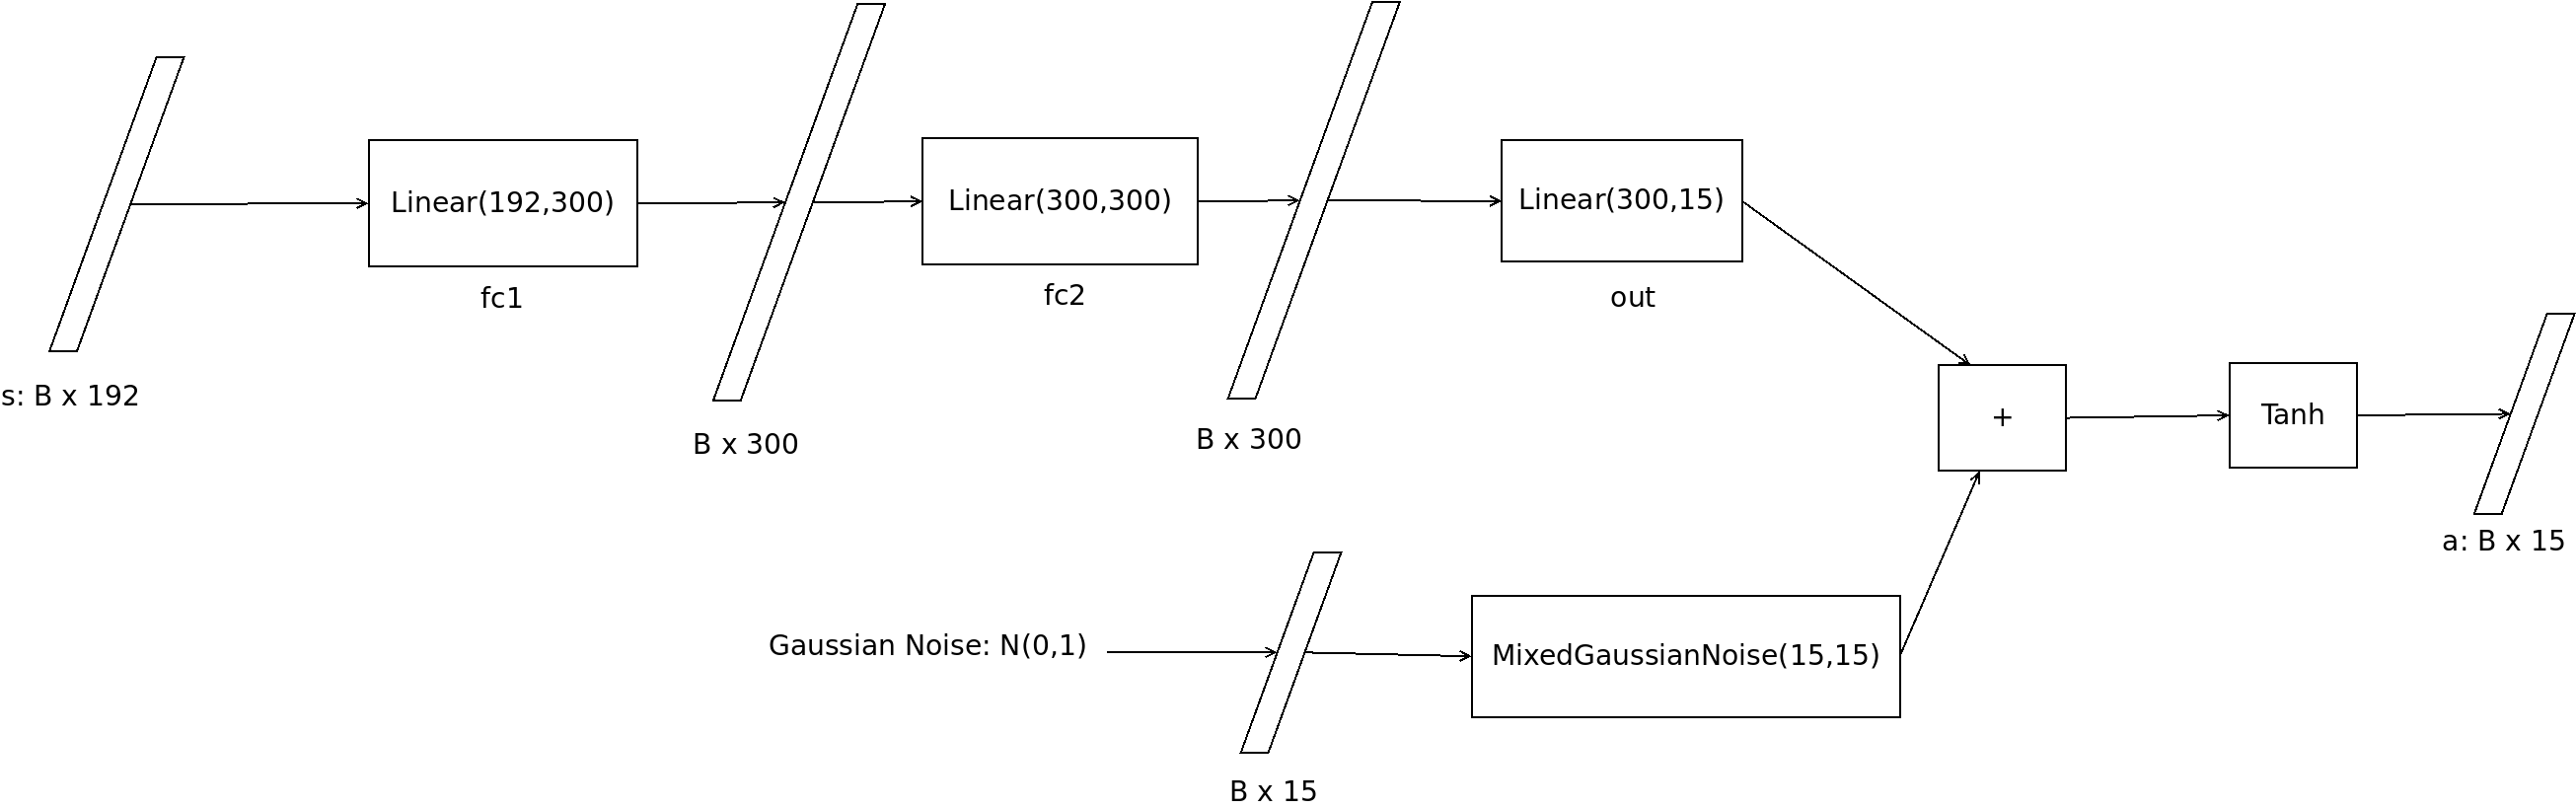
\includegraphics[width=\textwidth]{myenvMunet.png}
        \caption{Pyrobolearn中主体实验演员网络结构}
        \label{myenvMunet}
    \end{figure}

    \begin{figure}
        \centering
        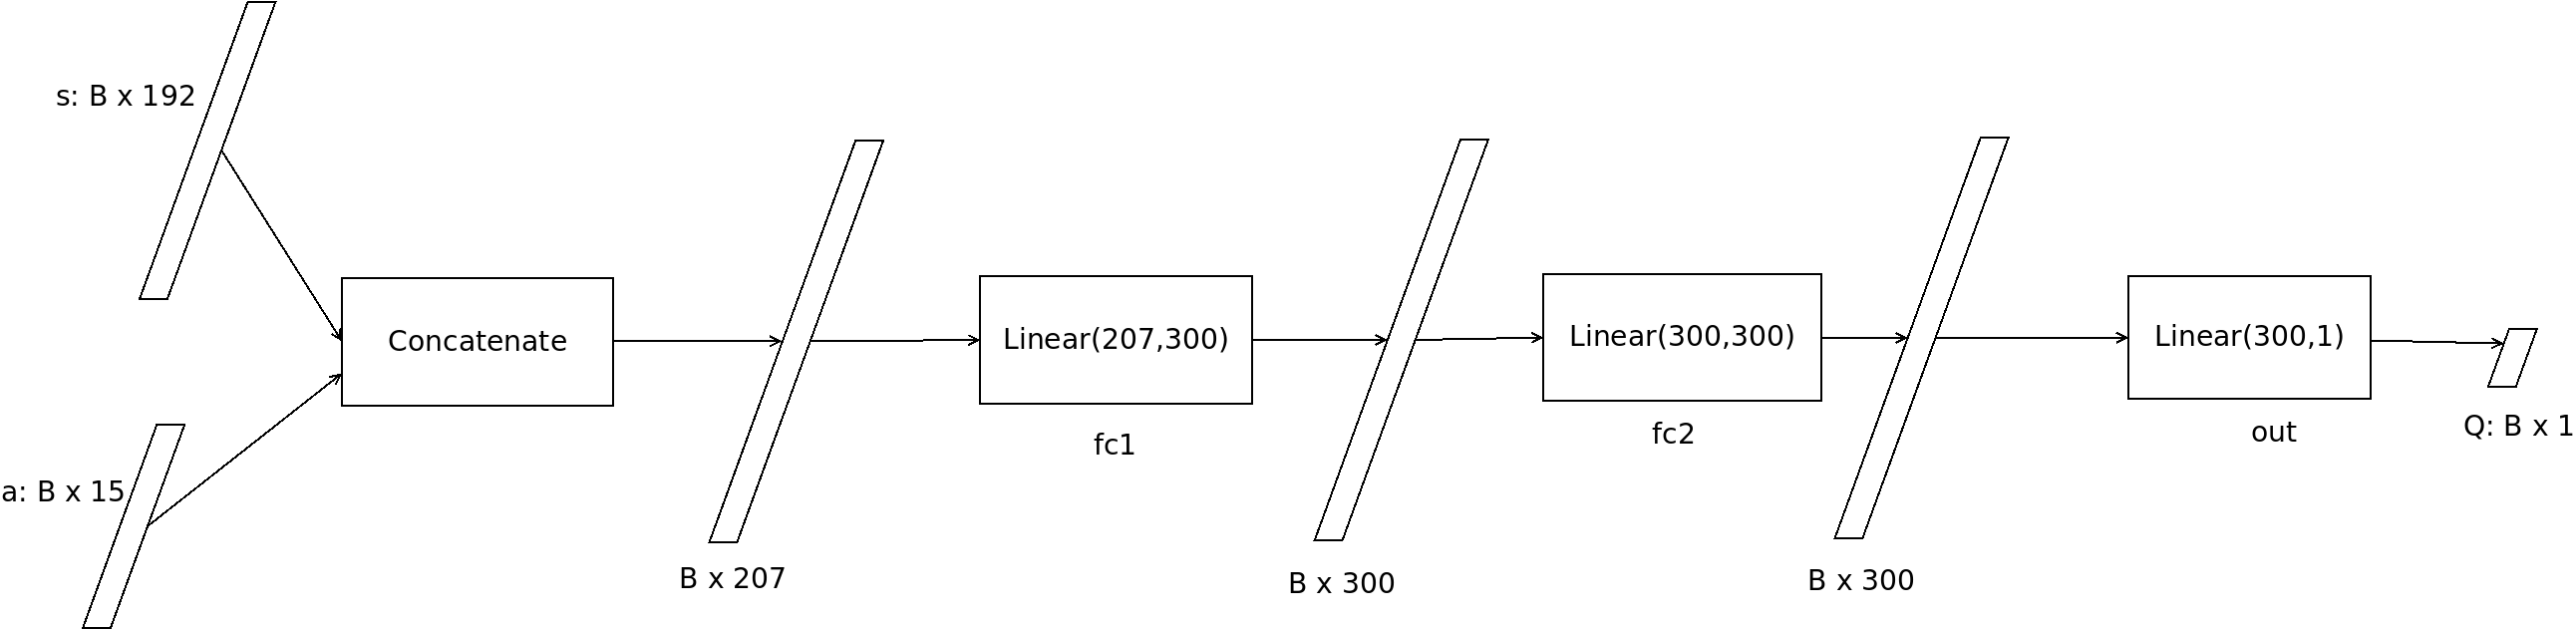
\includegraphics[width=\textwidth]{myenvQnet.png}
        \caption{Pyrobolearn中主体实验评论家网络结构}
        \label{myenvQnet}
    \end{figure}
% Local Variables:
% TeX-master: "../main"
% TeX-engine: xetex
% End:

\chapter{混合高斯噪声层}

\section{工作原理}
通常情况下,为了增加策略的稳健性,会对演员网络输出的动作向量添加一个均值为0,标准差为定值的高斯噪声。得到的动作常常还要进行裁剪以防止出现不合理的动作。然而,此种方法需要对两个超参数进行调节,需要大量的时间来进行训练,寻找最优的超参数值。由于在此主体实验中,往往需要训练很长的时间,因此引入这两个超参数并不理想。
    
为了避免手动调节噪声大小,本文提出了一个嵌入演员网络的可自动调节的混合高斯噪声。这个自动调节的噪声向量是通过直接在正态噪声向量后添加全连接层来得到的。得到的噪声向量被加到演员网络最后一层的输出上。
形式化地,给定一个从正态分布中随机采样的$B\times \mathrm{dim}(a)$的高斯噪声矩阵$X_{B\times \mathrm{dim}(a)}$,其中$B$是训练的迁移批次大小,$\mathrm{dim}(a)$是动作空间的维度大小。
如果把演员网络中确定性的部分的输出表示为$f(s)$,其中$s$是输入的状态向量,则有如下缩放后的噪声:

    $$ \mu(s) = f(s) + W X + b, X_{ij}\sim\mathcal N(0,1),$$

    其中$W$和$b$是全连接层的权重,它们通过反向传播自动调节。

\section{实验设计}
    为了更好地展示添加此混合高斯噪声层的效果,研究中在Pyrobolearn中的自定义环境中进行了两个实验以进行对照。其中一个有着固定的噪声大小作为超参数,而另一个没有此超参数而是换成了本文提出的混合高斯噪声层。
    实验系统的基本设计已经在\ref{myenvexp}中进行了详细讨论。本实验中使用了\ref{td3sec}中描述的未来替换方法,与\ref{myenvexp}中不同的是,在这两个实验中对每个网络都多添加了一层隐藏层。此外,随机初始化时对蓝色方块使用了$x,y\in[-1,1]$的均匀采样,WAM机械臂的最后一个末端执行器与方块的距离达到0.5米以内即可获得0.0的奖励,其余情况获得-1.0的奖励,且对靶网络的更新每2个片段进行一次。使用的实验参数如表\ref{fcntable}所示,其中符号的意义与\ref{pretable}中相同。

    \begin{table}[htbp]
        \caption{混合高斯噪声层实验参数}
        \label{fcntable}
    \vspace{0.5em}\centering\wuhao
    \begin{tabular}{ccccc}
    \toprule[1.5pt]
    实验参数 & 值\\
    \midrule[1pt]
        $\epsilon_{noise}$ & 0.2\\
        $\sigma_{clip}$ & 0.5\\
        $M$ & $5\times 10^3$\\
        $\epsilon_{rand}$ & 0.3\\
        $\gamma$ & 0.991\\
        $\alpha$ & $3\times 10^{-4}$\\
        $B$ & 16\\
        $\tau$ & 0.005\\
        $T$ & 50\\
        $f_\mu$ & 2\\
        $T_{start}$ & $2.5\times 10^4$\\
        $N_{sample}$ & 200 \\
        $k$ & 18\\
        $K_{replay}$ & 4\\
        $\xi_{LSH}$ & $2\times 10^{-2}$\\
    \bottomrule[1.5pt]
    \end{tabular}
    \end{table}
    其中$k$是\ref{LSHsec}中的超参数,用于调整对状态空间离散化的粒度。
    $K_{replay}$是\ref{HERsec}中所述的超参数,它与替换掉的迁移的比例有关。
    $\xi_{LSH}$是在计算最终奖励时,基于局部敏感哈希和计数的探索奖励的系数。
    其余参数的意义与表\ref{pretable}中相同。

\section{实验结果与分析}
    平均每个片段的使用混合高斯噪声层的演员网络的损失和使用噪声大小超参数的演员网络的损失如图\ref{fcn_lossmu}所示。有混合高斯噪声层的演员网络的损失在较少的代数内上升到了一个相对较低的值。由于这两组实验中损失都收敛到了较高的值,此损失曲线并不能明确反映哪种方法更优,因为演员网络的损失是由评论家网络决定的,而这两组实验中的评论家并不一定具有相同权重,因此即使是相同的演员网络也有可能具有不同的损失。

        \begin{figure}[htpb]
        \centering
        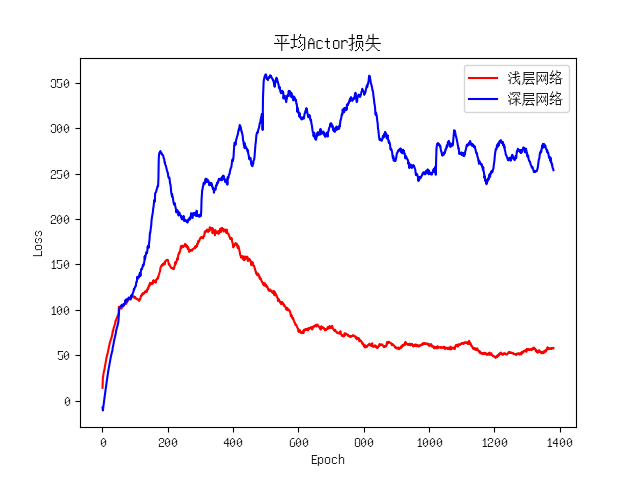
\includegraphics[width=0.6\textwidth]{myenv_lossmu.png}
        \caption{演员网络$\mu$的损失曲线}
            \label{fcn_lossmu}
        \end{figure}

    每个片段的评论家网络$Q_1$和$Q_2$的平均损失分别如图\ref{fcn_lossq1}和图\ref{fcn_lossq2}所示。可以看出,它们的损失也是和演员网络$\mu$的损失具有相似的形状。由于评论家网络的损失也并没有收敛到较低的值,这些损失曲线也不能反映混合高斯噪声层带来的变化。但是可以肯定的是,添加混合高斯噪声层后损失曲线变化更加平缓了。从图中也可以看出,评论家网络的损失比演员网络的损失更加不稳定,这可能是由于评论家网络的损失直接与环境相关导致的。

        \begin{figure}[htpb]
        \centering
        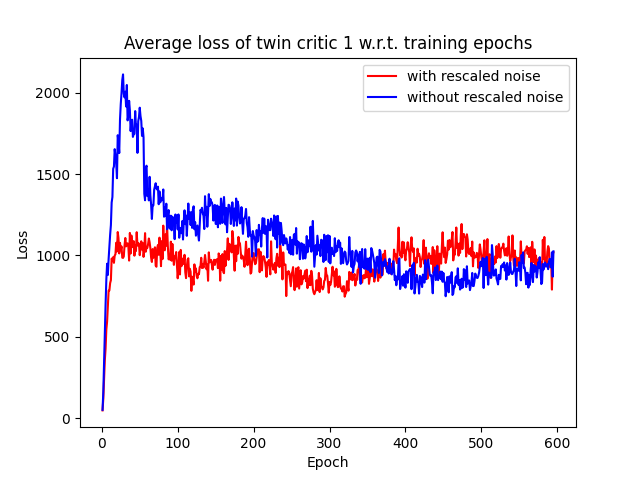
\includegraphics[width=0.6\textwidth]{myenv_lossq1.png}
        \caption{评论家网络$Q_1$的损失曲线}
            \label{fcn_lossq1}
        \end{figure}

        \begin{figure}[htpb]
        \centering
        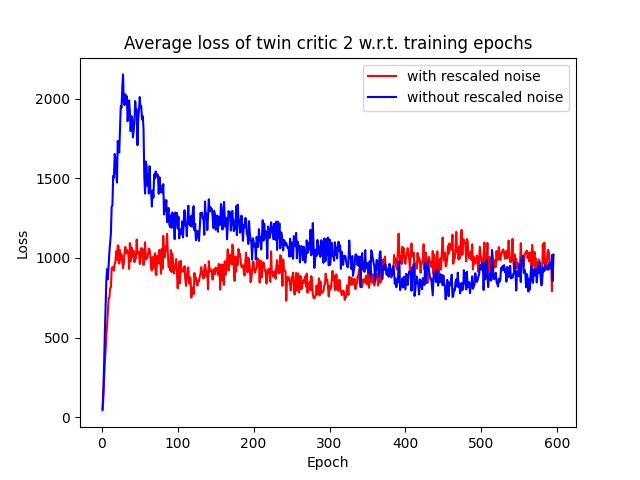
\includegraphics[width=0.6\textwidth]{myenv_lossq2.png}
        \caption{评论家网络$Q_2$的损失曲线}
            \label{fcn_lossq2}
        \end{figure}

        使用和不使用混合高斯噪声层的单位片段平均环境奖励如图\ref{fcn_reward}所示。可以看出,添加了混合高斯噪声层的方法获得的奖励要稍微比只使用噪声大小超参数的方法更高。

        \begin{figure}[htpb]
        \centering
        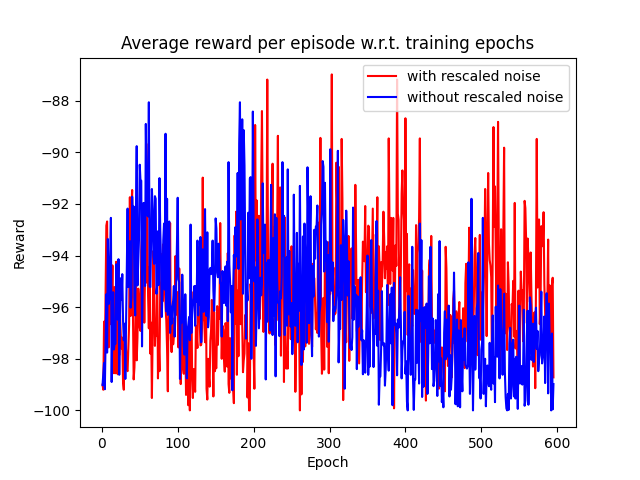
\includegraphics[width=0.6\textwidth]{myenv_reward.png}
        \caption{平均环境奖励曲线}
            \label{fcn_reward}
        \end{figure}

        平均成功率曲线的变化趋势与平均环境奖励的大致相同。对于最后的平均成功率,添加了混合高斯噪声层的要稍微更高。

        \begin{figure}[htpb]
        \centering
        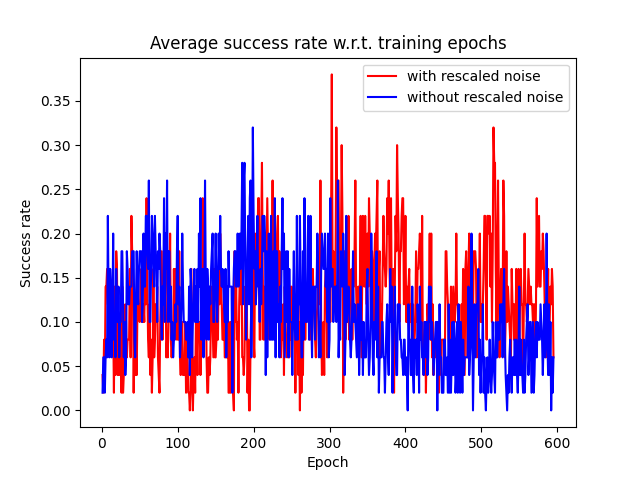
\includegraphics[width=0.6\textwidth]{myenv_suc_rate.png}
        \caption{任务目标成功率}
            \label{fcn_suc_rate}
        \end{figure}


\chapter{仿真时间奖励}

\section{工作原理}
在对物理过程进行仿真的过程中,物理引擎往往会做一些缓存和优化来对仿真进行加速,而这种加速是基于此物理过程容易预测这一事实的。这意味着,对于难以进行预测的复杂物理行为,如复杂的碰撞,物理引擎要消耗更多的时间来进行仿真。这就使得利用此信息来为智能体提供任务无关的探索奖励成为可能。

在实验过程中,为了准确计算仿真时间,避免其他因素影响,必须保证在训练过程中没有其他程序在运行。这一要求可以简单地通过避免在训练时操作计算机来满足。此外,为了防止系统调用的时间被计入,在实验中对仿真时间进行计算时,直接在仿真代码被调用前后使用Python的time库进行了计时。

除了仿真时间奖励外,实验中还提供了基于局部敏感哈希的探索奖励。为了平衡不同的内部奖励,需要在计算最终奖励前先乘上一个系数。

在演员网络中,使用了上一章提出的混合高斯噪声层,但不同的是,为了防止噪声产生过大影响,继续使用参数$\sigma_{clip}$对噪声进行裁剪。

为了防止机械臂在可以完成任务的动作序列中选择较长的序列,在对演员网络进行优化时,可以在其损失函数中添加一个动作惩罚项,即

   $$ L_\mu = -\sum_i^N\frac{Q_1(s_i, \mu(s_i))}{N} + \xi_{action}||\mu(s_i)||^2$$
其中$\xi_{action}$是动作惩罚系数。

在实验中,整个系统都采用\ref{myenvexp}中的设计,但是除了使用\ref{myenvexp}中的浅层网络结构外,还增加了一个为每个网络添加一个隐藏层的深层网络作为对照组。

由于在使用正向动力学预测模型来计算奖励时,会导致训练速度极大下降,而且在实验中并未发现它能够对算法结果产生有利影响,因此在本章实验中不再展示相关的实验结果和数据。

实验相关的参数见表\ref{simtable}。
    \begin{table}[htbp]
        \caption{仿真时间奖励实验参数}
        \label{simtable}
    \vspace{0.5em}\centering\wuhao
    \begin{tabular}{ccccc}
    \toprule[1.5pt]
    实验参数 & 值\\
    \midrule[1pt]
        $\sigma_{clip}$ & 0.5\\
        $M$ & 300\\
        $\epsilon_{rand}$ & 0.3\\
        $\xi_{action}$ & $1\times 10^{-3}$\\
        $\gamma$ & 0.998\\
        $\alpha$ & $1\times 10^{-3}$\\
        $B$ & 10000\\
        $\tau$ & 0.23\\
        $T$ & 200\\
        $N_{batches}$ & 1\\
        $f_{target}$ & 200\\
        $f_{actor}$ & 400\\
        $f_{critic}$ & 200\\
        $T_{start}$ & $1\times 10^5$\\
        $N_{sample}$ & 50 \\
        $k$ & 18\\
        $K_{replay}$ & 4\\
        $\xi_{LSH}$ & $2\times 10^{-2}$\\
        $\xi_{sim}$ & 10\\
    \bottomrule[1.5pt]
    \end{tabular}
    \end{table}
    其中$\xi_{action}$是动作惩罚系数,$N_{batches}$指每次触发对演员网络或评论家网络的训练时迭代的次数。
    每经过$f_{target}$个时间步,使用指数滑动平均对靶网络进行权重更新。
    每经过$f_{actor}$个时间步,使用反向传播对演员网络权重进行更新。
    每经过$f_{critic}$个时间步,使用优化器对评论家网络权重进行更新。
    $\xi_{sim}$是在计算最终奖励时,仿真时间奖励的系数。
    其余的参数意义与表\ref{fcntable}中相同。
\section{实验结果与分析}

只有3层与有4层的网络相比,演员网络损失曲线如图\ref{simlossmu}所示。可以看出浅层网络更快地收敛了,而深层网络收敛到了一个损失较大的值。
        \begin{figure}[htpb]
        \centering
        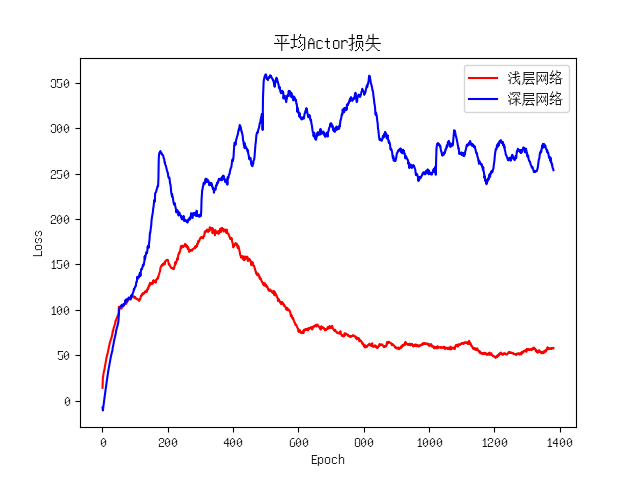
\includegraphics[width=0.6\textwidth]{sim_myenv_lossmu.png}
        \caption{3层和4层演员网络$\mu$的损失曲线}
            \label{simlossmu}
        \end{figure}

对于评论家网络来说,如图\ref{simlossq1}和\ref{simlossq2}所示,情况是类似的,更加值得注意的是,深层网络更容易出现损失突然暴增的现象,这意味着深层网络训练起来更加不稳定。
        \begin{figure}[htpb]
        \centering
        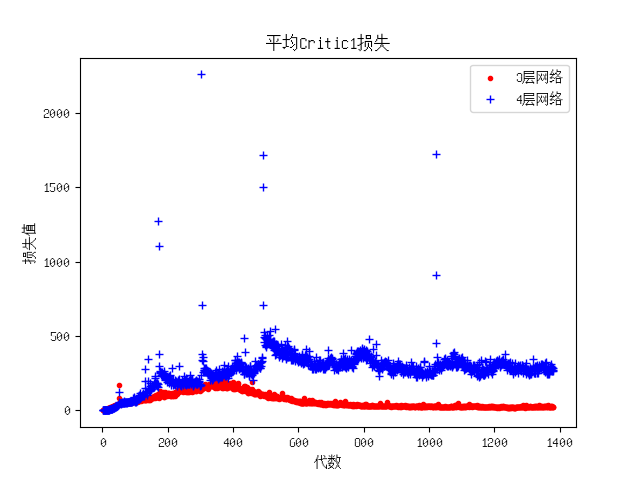
\includegraphics[width=0.6\textwidth]{sim_myenv_lossq1.png}
        \caption{3层和4层评论家网络$Q_1$的损失曲线}
            \label{simlossq1}
        \end{figure}

        \begin{figure}[htpb]
        \centering
        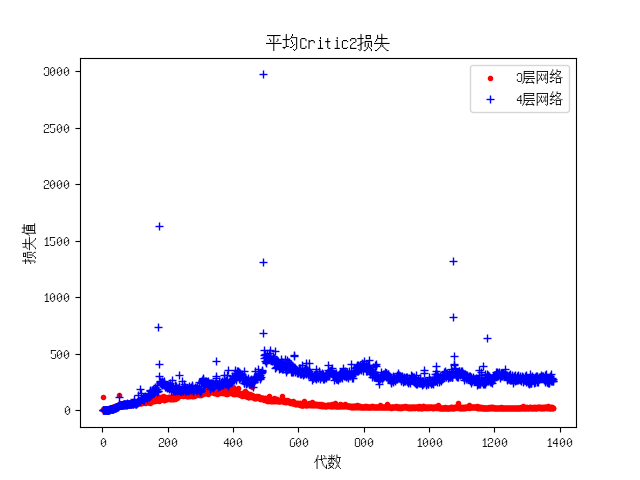
\includegraphics[width=0.6\textwidth]{sim_myenv_lossq2.png}
        \caption{3层和4层评论家网络$Q_2$的损失曲线}
            \label{simlossq2}
        \end{figure}

浅层网络和深层网络的平均环境奖励如图\ref{simenv_reward}所示,可以看出浅层最后学习到了一个较好的策略,得到的奖励显著比深层网络更高,而深层网络的奖励一直维持在最差的结果附近。

        \begin{figure}[htpb]
        \centering
        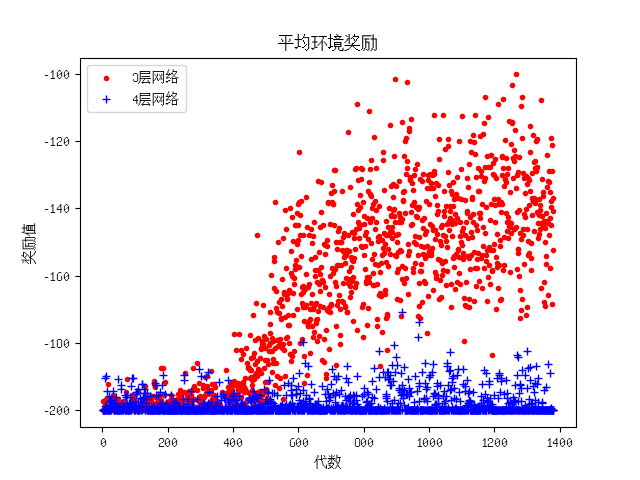
\includegraphics[width=0.6\textwidth]{sim_myenv_reward.png}
        \caption{浅层神经网络和深层神经网络的平均环境奖励曲线}
            \label{simenv_reward}
        \end{figure}

观察图\ref{simlsh_reward}中所示的基于局部敏感哈希的计数奖励可以发现,浅层网络的基于局部敏感哈希的计数奖励与深层网络的相差不多,甚至在200代附近深层网络反而获得了更高的奖励。

        \begin{figure}[htpb]
        \centering
        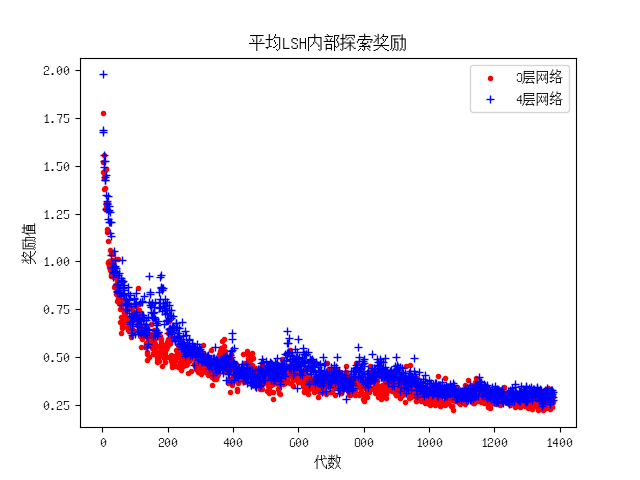
\includegraphics[width=0.6\textwidth]{sim_myenv_lsh_reward.png}
        \caption{浅层网络和深层网络的基于局部敏感哈希的平均计数奖励曲线}
            \label{simlsh_reward}
        \end{figure}
而仿真时间奖励则能比基于局部敏感哈希的计数奖励更好地反映策略的好坏,如图\ref{simsim_reward}所示,仿真时间奖励在900代之后浅层网络要比深层网络更高,这与环境奖励的趋势吻合,表明仿真时间奖励不仅具有任务无关的鼓励智能体探索的能力,还能帮助智能体在探索之后策略泛化到给定开放任务中。

        \begin{figure}[htpb]
        \centering
        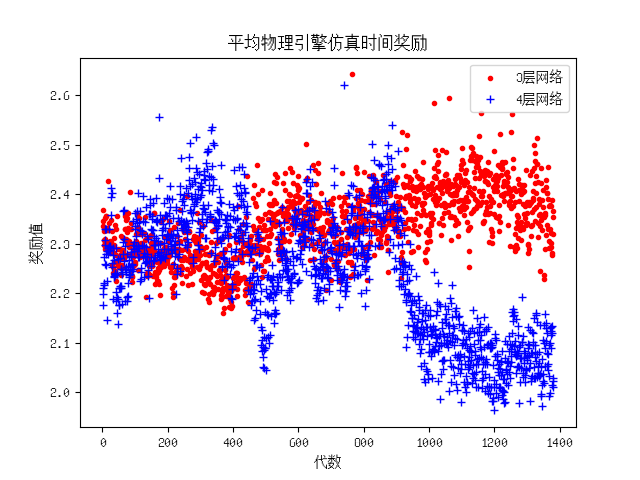
\includegraphics[width=0.6\textwidth]{sim_myenv_sim_reward.png}
        \caption{浅层网络和深层网络的平均仿真时间奖励曲线}
            \label{simsim_reward}
        \end{figure}
图\ref{simsuc_rate}中的成功率变化与环境奖励的变化趋势相似,这和在其他实验中观察到的一致。

        \begin{figure}[htpb]
        \centering
        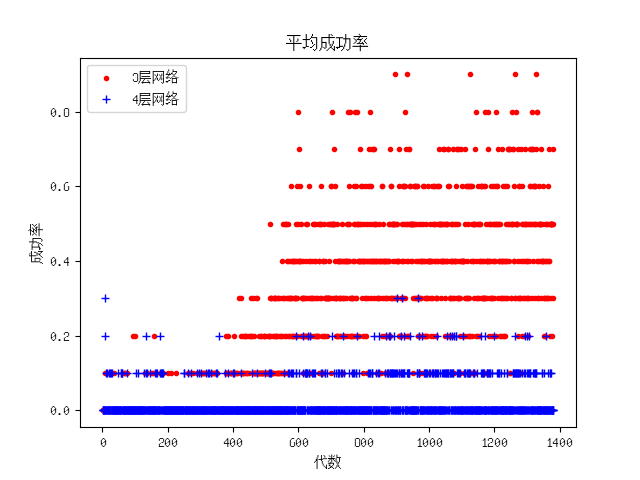
\includegraphics[width=0.6\textwidth]{sim_myenv_suc_rate.png}
        \caption{浅层网络和深层网络平均任务目标成功率曲线}
            \label{simsuc_rate}
        \end{figure}
在对深层网络的梯度进行观测时,可以观察到演员网络中的梯度快速地减小至0,这意味着发生了梯度消失,如果使用残差网络、层归一化或进行谱归一化,则有可能进一步提高性能。

在训练完成后,智能体完成接近方块的开放任务的成功率约为60\%,如图\ref{reach}所示为智能体成功完成任务时的截图。

        \begin{figure}[htpb]
        \centering
        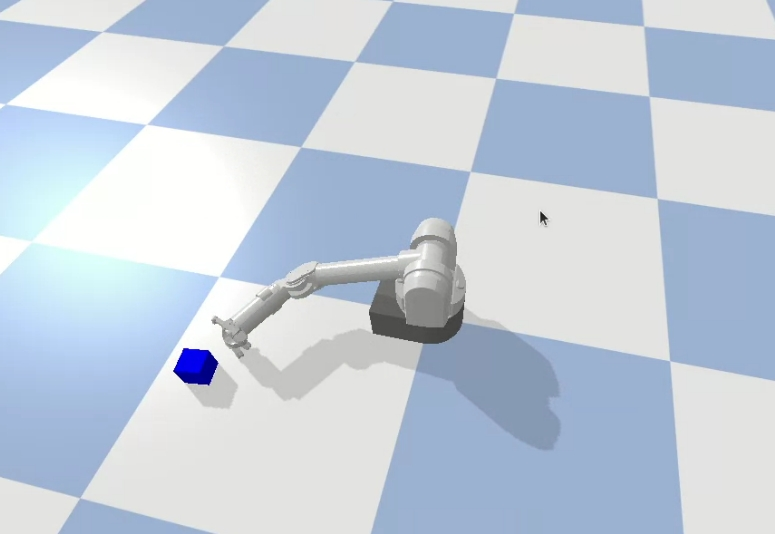
\includegraphics[width=0.6\textwidth]{reach.jpg}
        \caption{机械臂智能体完成任务的结果展示}
            \label{reach}
        \end{figure}

\backmatter
% !Mode:: "TeX:UTF-8" 
\begin{conclusions}

    本文结合了TD3算法、HER算法和基于LSH和计数的奖励、基于正向动力学预测的奖励,并提出了混合高斯噪声层和将物理仿真时间作为于未知任务的探索奖励。本文中的算法可以很好地用于训练可适应到给定开放任务的智能体,表现出与现有探索奖励相当的性能。
\end{conclusions}
   % 结论
\bibliographystyle{hithesis} %如果没有参考文献时候
\bibliography{reference}
%%%%%%%%%%%%%%%%%%%%%%%%%%%%%%%%%%%%%%%%%%%%%%%%%%%%%%%%%%%%%%%%%%%%%%%%%%%%%%%% 
%-- 注意:以下本硕博、博后书序不一致 --%
%%%%%%%%%%%%%%%%%%%%%%%%%%%%%%%%%%%%%%%%%%%%%%%%%%%%%%%%%%%%%%%%%%%%%%%%%%%%%%%% 
% 硕博书序
%%%%%%%%%%%%%%%%%%%%%%%%%%%%%%%%%%%%%%%%%%%%%%%%%%%%%%%%%%%%%%%%%%%%%%%%%%%%%%%% 
\begin{appendix}%附录
% -*-coding: utf-8 -*-
%%%%%%%%%%%%%%%%%%%%%%%%%%%%%%%%%%%%%%%%%%%%%%%%%%%%%%%%%
\chapter{算法代码}

%%%%%%%%%%%%%%%%%%%%%%%%%%%%%%%%%%%%%%%%%%%%%%%%%%%%%%%%%
\section{训练代码}

\section{测试代码}

\end{appendix}
\begin{ceindex}
  %如果想要手动加索引,注释掉以下这一样,用wordlist环境
\printsubindex*
\end{ceindex}
    % 索引, 根据自己的情况添加或者不添加,选择自动添加或者手工添加。
\authorization %授权
%\authorization[scan.pdf] %添加扫描页的命令,与上互斥
% !Mode:: "TeX:UTF-8"
\begin{acknowledgements}
衷心感谢导师~范晓鹏~教授对本人的精心指导。他的言传身教将使我终生受益。

感谢哈工大\LaTeX\ 论文模板\hithesis\ 。

\end{acknowledgements}
 %致谢
%%%%%%%%%%%%%%%%%%%%%%%%%%%%%%%%%%%%%%%%%%%%%%%%%%%%%%%%%%%%%%%%%%%%%%%%%%%%%%%% 
% 本科书序为:
%%%%%%%%%%%%%%%%%%%%%%%%%%%%%%%%%%%%%%%%%%%%%%%%%%%%%%%%%%%%%%%%%%%%%%%%%%%%%%%% 
% \authorization %授权
% % \authorization[scan.pdf] %添加扫描页的命令,与上互斥
% % !Mode:: "TeX:UTF-8"
\begin{acknowledgements}
衷心感谢导师~范晓鹏~教授对本人的精心指导。他的言传身教将使我终生受益。

感谢哈工大\LaTeX\ 论文模板\hithesis\ 。

\end{acknowledgements}
 %致谢
% \begin{appendix}%附录
% \chapter{外文资料原文}
\label{cha:engorg}

\title{The title of the English paper}

\textbf{Abstract:} As one of the most widely used techniques in operations
research, \emph{ mathematical programming} is defined as a means of maximizing a
quantity known as \emph{bjective function}, subject to a set of constraints
represented by equations and inequalities. Some known subtopics of mathematical
programming are linear programming, nonlinear programming, multiobjective
programming, goal programming, dynamic programming, and multilevel
programming$^{[1]}$.

It is impossible to cover in a single chapter every concept of mathematical
programming. This chapter introduces only the basic concepts and techniques of
mathematical programming such that readers gain an understanding of them
throughout the book$^{[2,3]}$.


\section{Single-Objective Programming}
The general form of single-objective programming (SOP) is written
as follows,
\begin{equation}\tag*{(123)} % 如果附录中的公式不想让它出现在公式索引中,那就请
                             % 用 \tag*{xxxx}
\left\{\begin{array}{l}
\max \,\,f(x)\\[0.1 cm]
\mbox{subject to:} \\ [0.1 cm]
\qquad g_j(x)\le 0,\quad j=1,2,\cdots,p
\end{array}\right.
\end{equation}
which maximizes a real-valued function $f$ of
$x=(x_1,x_2,\cdots,x_n)$ subject to a set of constraints.

\newtheorem{mpdef}{Definition}[chapter]
\begin{mpdef}
In SOP, we call $x$ a decision vector, and
$x_1,x_2,\cdots,x_n$ decision variables. The function
$f$ is called the objective function. The set
\begin{equation}\tag*{(456)} % 这里同理,其它不再一一指定。
S=\left\{x\in\Re^n\bigm|g_j(x)\le 0,\,j=1,2,\cdots,p\right\}
\end{equation}
is called the feasible set. An element $x$ in $S$ is called a
feasible solution.
\end{mpdef}

\newtheorem{mpdefop}[mpdef]{Definition}
\begin{mpdefop}
A feasible solution $x^*$ is called the optimal
solution of SOP if and only if
\begin{equation}
f(x^*)\ge f(x)
\end{equation}
for any feasible solution $x$.
\end{mpdefop}

One of the outstanding contributions to mathematical programming was known as
the Kuhn-Tucker conditions\ref{eq:ktc}. In order to introduce them, let us give
some definitions. An inequality constraint $g_j(x)\le 0$ is said to be active at
a point $x^*$ if $g_j(x^*)=0$. A point $x^*$ satisfying $g_j(x^*)\le 0$ is said
to be regular if the gradient vectors $\nabla g_j(x)$ of all active constraints
are linearly independent.

Let $x^*$ be a regular point of the constraints of SOP and assume that all the
functions $f(x)$ and $g_j(x),j=1,2,\cdots,p$ are differentiable. If $x^*$ is a
local optimal solution, then there exist Lagrange multipliers
$\lambda_j,j=1,2,\cdots,p$ such that the following Kuhn-Tucker conditions hold,
\begin{equation}
\label{eq:ktc}
\left\{\begin{array}{l}
    \nabla f(x^*)-\sum\limits_{j=1}^p\lambda_j\nabla g_j(x^*)=0\\[0.3cm]
    \lambda_jg_j(x^*)=0,\quad j=1,2,\cdots,p\\[0.2cm]
    \lambda_j\ge 0,\quad j=1,2,\cdots,p.
\end{array}\right.
\end{equation}
If all the functions $f(x)$ and $g_j(x),j=1,2,\cdots,p$ are convex and
differentiable, and the point $x^*$ satisfies the Kuhn-Tucker conditions
(\ref{eq:ktc}), then it has been proved that the point $x^*$ is a global optimal
solution of SOP.

\subsection{Linear Programming}
\label{sec:lp}

If the functions $f(x),g_j(x),j=1,2,\cdots,p$ are all linear, then SOP is called
a {\em linear programming}.

The feasible set of linear is always convex. A point $x$ is called an extreme
point of convex set $S$ if $x\in S$ and $x$ cannot be expressed as a convex
combination of two points in $S$. It has been shown that the optimal solution to
linear programming corresponds to an extreme point of its feasible set provided
that the feasible set $S$ is bounded. This fact is the basis of the {\em simplex
  algorithm} which was developed by Dantzig as a very efficient method for
solving linear programming.
\begin{table}[ht]
\centering
  \centering
  \caption*{Table~1\hskip1em This is an example for manually numbered table, which
    would not appear in the list of tables}
  \label{tab:badtabular2}
  \begin{tabular}[c]{|m{1.5cm}|c|c|c|c|c|c|}\hline
    \multicolumn{2}{|c|}{Network Topology} & \# of nodes &
    \multicolumn{3}{c|}{\# of clients} & Server \\\hline
    GT-ITM & Waxman Transit-Stub & 600 &
    \multirow{2}{2em}{2\%}&
    \multirow{2}{2em}{10\%}&
    \multirow{2}{2em}{50\%}&
    \multirow{2}{1.2in}{Max. Connectivity}\\\cline{1-3}
    \multicolumn{2}{|c|}{Inet-2.1} & 6000 & & & &\\\hline
    & \multicolumn{2}{c|}{ABCDEF} &\multicolumn{4}{c|}{} \\\hline
\end{tabular}
\end{table}

Roughly speaking, the simplex algorithm examines only the extreme points of the
feasible set, rather than all feasible points. At first, the simplex algorithm
selects an extreme point as the initial point. The successive extreme point is
selected so as to improve the objective function value. The procedure is
repeated until no improvement in objective function value can be made. The last
extreme point is the optimal solution.

\subsection{Nonlinear Programming}

If at least one of the functions $f(x),g_j(x),j=1,2,\cdots,p$ is nonlinear, then
SOP is called a {\em nonlinear programming}.

A large number of classical optimization methods have been developed to treat
special-structural nonlinear programming based on the mathematical theory
concerned with analyzing the structure of problems.

Now we consider a nonlinear programming which is confronted solely with
maximizing a real-valued function with domain $\Re^n$.  Whether derivatives are
available or not, the usual strategy is first to select a point in $\Re^n$ which
is thought to be the most likely place where the maximum exists. If there is no
information available on which to base such a selection, a point is chosen at
random. From this first point an attempt is made to construct a sequence of
points, each of which yields an improved objective function value over its
predecessor. The next point to be added to the sequence is chosen by analyzing
the behavior of the function at the previous points. This construction continues
until some termination criterion is met. Methods based upon this strategy are
called {\em ascent methods}, which can be classified as {\em direct methods},
{\em gradient methods}, and {\em Hessian methods} according to the information
about the behavior of objective function $f$. Direct methods require only that
the function can be evaluated at each point. Gradient methods require the
evaluation of first derivatives of $f$. Hessian methods require the evaluation
of second derivatives. In fact, there is no superior method for all
problems. The efficiency of a method is very much dependent upon the objective
function.

\subsection{Integer Programming}

{\em Integer programming} is a special mathematical programming in which all of
the variables are assumed to be only integer values. When there are not only
integer variables but also conventional continuous variables, we call it {\em
  mixed integer programming}. If all the variables are assumed either 0 or 1,
then the problem is termed a {\em zero-one programming}. Although integer
programming can be solved by an {\em exhaustive enumeration} theoretically, it
is impractical to solve realistically sized integer programming problems. The
most successful algorithm so far found to solve integer programming is called
the {\em branch-and-bound enumeration} developed by Balas (1965) and Dakin
(1965). The other technique to integer programming is the {\em cutting plane
  method} developed by Gomory (1959).

\hfill\textit{Uncertain Programming\/}\quad(\textsl{BaoDing Liu, 2006.2})

\section*{References}
\noindent{\itshape NOTE: These references are only for demonstration. They are
  not real citations in the original text.}

\begin{translationbib}
\item Donald E. Knuth. The \TeX book. Addison-Wesley, 1984. ISBN: 0-201-13448-9
\item Paul W. Abrahams, Karl Berry and Kathryn A. Hargreaves. \TeX\ for the
  Impatient. Addison-Wesley, 1990. ISBN: 0-201-51375-7
\item David Salomon. The advanced \TeX book.  New York : Springer, 1995. ISBN:0-387-94556-3
\end{translationbib}

\chapter{外文资料的调研阅读报告或书面翻译}

\title{英文资料的中文标题}

{\heiti 摘要:} 本章为外文资料翻译内容。如果有摘要可以直接写上来,这部分好像没有
明确的规定。

\section{单目标规划}
北冥有鱼,其名为鲲。鲲之大,不知其几千里也。化而为鸟,其名为鹏。鹏之背,不知其几
千里也。怒而飞,其翼若垂天之云。是鸟也,海运则将徙于南冥。南冥者,天池也。
\begin{equation}\tag*{(123)}
 p(y|\mathbf{x}) = \frac{p(\mathbf{x},y)}{p(\mathbf{x})}=
\frac{p(\mathbf{x}|y)p(y)}{p(\mathbf{x})}
\end{equation}

吾生也有涯,而知也无涯。以有涯随无涯,殆已!已而为知者,殆而已矣!为善无近名,为
恶无近刑,缘督以为经,可以保身,可以全生,可以养亲,可以尽年。

\subsection{线性规划}
庖丁为文惠君解牛,手之所触,肩之所倚,足之所履,膝之所倚,砉然响然,奏刀騞然,莫
不中音,合于桑林之舞,乃中经首之会。
\begin{table}[ht]
\centering
  \centering
  \caption*{表~1\hskip1em 这是手动编号但不出现在索引中的一个表格例子}
  \label{tab:badtabular3}
  \begin{tabular}[c]{|m{1.5cm}|c|c|c|c|c|c|}\hline
    \multicolumn{2}{|c|}{Network Topology} & \# of nodes &
    \multicolumn{3}{c|}{\# of clients} & Server \\\hline
    GT-ITM & Waxman Transit-Stub & 600 &
    \multirow{2}{2em}{2\%}&
    \multirow{2}{2em}{10\%}&
    \multirow{2}{2em}{50\%}&
    \multirow{2}{1.2in}{Max. Connectivity}\\\cline{1-3}
    \multicolumn{2}{|c|}{Inet-2.1} & 6000 & & & &\\\hline
    & \multicolumn{2}{c|}{ABCDEF} &\multicolumn{4}{c|}{} \\\hline
\end{tabular}
\end{table}

文惠君曰:“嘻,善哉!技盖至此乎?”庖丁释刀对曰:“臣之所好者道也,进乎技矣。始臣之
解牛之时,所见无非全牛者;三年之后,未尝见全牛也;方今之时,臣以神遇而不以目视,
官知止而神欲行。依乎天理,批大郤,导大窾,因其固然。技经肯綮之未尝,而况大坬乎!
良庖岁更刀,割也;族庖月更刀,折也;今臣之刀十九年矣,所解数千牛矣,而刀刃若新发
于硎。彼节者有间而刀刃者无厚,以无厚入有间,恢恢乎其于游刃必有余地矣。是以十九年
而刀刃若新发于硎。虽然,每至于族,吾见其难为,怵然为戒,视为止,行为迟,动刀甚微,
謋然已解,如土委地。提刀而立,为之而四顾,为之踌躇满志,善刀而藏之。”

文惠君曰:“善哉!吾闻庖丁之言,得养生焉。”


\subsection{非线性规划}
孔子与柳下季为友,柳下季之弟名曰盗跖。盗跖从卒九千人,横行天下,侵暴诸侯。穴室枢
户,驱人牛马,取人妇女。贪得忘亲,不顾父母兄弟,不祭先祖。所过之邑,大国守城,小
国入保,万民苦之。孔子谓柳下季曰:“夫为人父者,必能诏其子;为人兄者,必能教其弟。
若父不能诏其子,兄不能教其弟,则无贵父子兄弟之亲矣。今先生,世之才士也,弟为盗
跖,为天下害,而弗能教也,丘窃为先生羞之。丘请为先生往说之。”

柳下季曰:“先生言为人父者必能诏其子,为人兄者必能教其弟,若子不听父之诏,弟不受
兄之教,虽今先生之辩,将奈之何哉?且跖之为人也,心如涌泉,意如飘风,强足以距敌,
辩足以饰非。顺其心则喜,逆其心则怒,易辱人以言。先生必无往。”

孔子不听,颜回为驭,子贡为右,往见盗跖。

\subsection{整数规划}
盗跖乃方休卒徒大山之阳,脍人肝而餔之。孔子下车而前,见谒者曰:“鲁人孔丘,闻将军
高义,敬再拜谒者。”谒者入通。盗跖闻之大怒,目如明星,发上指冠,曰:“此夫鲁国之
巧伪人孔丘非邪?为我告之:尔作言造语,妄称文、武,冠枝木之冠,带死牛之胁,多辞缪
说,不耕而食,不织而衣,摇唇鼓舌,擅生是非,以迷天下之主,使天下学士不反其本,妄
作孝弟,而侥幸于封侯富贵者也。子之罪大极重,疾走归!不然,我将以子肝益昼餔之膳。”


\chapter{其它附录}
前面两个附录主要是给本科生做例子。其它附录的内容可以放到这里,当然如果你愿意,可
以把这部分也放到独立的文件中,然后将其到主文件中。
%本科生翻译论文
% \end{appendix}
%%%%%%%%%%%%%%%%%%%%%%%%%%%%%%%%%%%%%%%%%%%%%%%%%%%%%%%%%%%%%%%%%%%%%%%%%%%%%%%% 
% 博后书序
%%%%%%%%%%%%%%%%%%%%%%%%%%%%%%%%%%%%%%%%%%%%%%%%%%%%%%%%%%%%%%%%%%%%%%%%%%%%%%%% 
% % !Mode:: "TeX:UTF-8"
\begin{acknowledgements}
衷心感谢导师~范晓鹏~教授对本人的精心指导。他的言传身教将使我终生受益。

感谢哈工大\LaTeX\ 论文模板\hithesis\ 。

\end{acknowledgements}
 %致谢
% % !Mode:: "TeX:UTF-8" 

\begin{doctorpublication}
\noindent\textbf{(一)发表的学术论文}
\begin{publist}
\item	XXX,XXX. Static Oxidation Model of Al-Mg/C Dissipation Thermal Protection Materials[J]. Rare Metal Materials and Engineering, 2010, 39(Suppl. 1): 520-524.(SCI~收录,IDS号为~669JS,IF=0.16)
\item XXX,XXX. 精密超声振动切削单晶铜的计算机仿真研究[J]. 系统仿真学报,2007,19(4):738-741,753.(EI~收录号:20071310514841)
\item XXX,XXX. 局部多孔质气体静压轴向轴承静态特性的数值求解[J]. 摩擦学学报,2007(1):68-72.(EI~收录号:20071510544816)
\item XXX,XXX. 硬脆光学晶体材料超精密切削理论研究综述[J]. 机械工程学报,2003,39(8):15-22.(EI~收录号:2004088028875)
\item XXX,XXX. 基于遗传算法的超精密切削加工表面粗糙度预测模型的参数辨识以及切削参数优化[J]. 机械工程学报,2005,41(11):158-162.(EI~收录号:2006039650087)
\item XXX,XXX. Discrete Sliding Mode Cintrok with Fuzzy Adaptive Reaching Law on 6-PEES Parallel Robot[C]. Intelligent System Design and Applications, Jinan, 2006: 649-652.(EI~收录号:20073210746529)
\end{publist}

\noindent\textbf{(二)申请及已获得的专利(无专利时此项不必列出)}
\begin{publist}
\item XXX,XXX. 一种温热外敷药制备方案:中国,88105607.3[P]. 1989-07-26.
\end{publist}

\noindent\textbf{(三)参与的科研项目及获奖情况}
\begin{publist}
\item	XXX,XXX. XX~气体静压轴承技术研究, XX~省自然科学基金项目.课题编号:XXXX.
\item XXX,XXX. XX~静载下预应力混凝土房屋结构设计统一理论. 黑江省科学技术二等奖, 2007.
\end{publist}
%\vfill
%\hangafter=1\hangindent=2em\noindent
%\setlength{\parindent}{2em}
\end{doctorpublication}
    % 所发文章
% % !Mode:: "TeX:UTF-8" 
\begin{publication}
\noindent\textbf{发表的相关论文}
\begin{publist}
\item	XXX,XXX. Static Oxidation Model of Al-Mg/C Dissipation Thermal Protection Materials[J]. Rare Metal Materials and Engineering, 2010, 39(Suppl. 1): 520-524.(SCI~收录,IDS号为~669JS,IF=0.16)
\item XXX,XXX. 精密超声振动切削单晶铜的计算机仿真研究[J]. 系统仿真学报,2007,19(4):738-741,753.(EI~收录号:20071310514841)
\item XXX,XXX. 局部多孔质气体静压轴向轴承静态特性的数值求解[J]. 摩擦学学报,2007(1):68-72.(EI~收录号:20071510544816)
\item XXX,XXX. 硬脆光学晶体材料超精密切削理论研究综述[J]. 机械工程学报,2003,39(8):15-22.(EI~收录号:2004088028875)
\item XXX,XXX. 基于遗传算法的超精密切削加工表面粗糙度预测模型的参数辨识以及切削参数优化[J]. 机械工程学报,2005,41(11):158-162.(EI~收录号:2006039650087)
\item XXX,XXX. Discrete Sliding Mode Cintrok with Fuzzy Adaptive Reaching Law on 6-PEES Parallel Robot[C]. Intelligent System Design and Applications, Jinan, 2006: 649-652.(EI~收录号:20073210746529)
\end{publist}

\noindent\textbf{(二)申请及已获得的专利(无专利时此项不必列出)}
\begin{publist}
\item XXX,XXX. 一种温热外敷药制备方案:中国,88105607.3[P]. 1989-07-26.
\end{publist}

\noindent\textbf{(三)参与的科研项目及获奖情况}
\begin{publist}
\item	XXX,XXX. XX~气体静压轴承技术研究, XX~省自然科学基金项目.课题编号:XXXX.
\item XXX,XXX. XX~静载下预应力混凝土房屋结构设计统一理论. 黑江省科学技术二等奖, 2007.
\end{publist}
%\vfill
%\hangafter=1\hangindent=2em\noindent
%\setlength{\parindent}{2em}
\end{publication}
    % 所发文章
% \include{back/resume}          % 博士学位论文有个人简介
% % !Mode:: "TeX:UTF-8"
\begin{correspondingaddr}
  \heiti\xiaosi
  \noindent 永久通讯地址: \par
  \noindent email: \par
  \noindent 电话: \par
\end{correspondingaddr}
 %通信地址
%%%%%%%%%%%%%%%%%%%%%%%%%%%%%%%%%%%%%%%%%%%%%%%%%%%%%%%%%%%%%%%%%%%%%%%%%%%%%%%% 
\end{document}
% Local Variables:
% TeX-engine: xetex
% End:
